\documentclass[12pt,a4paper,oneside]{book}
\input{khaibao}

\begin{document}
	\thispagestyle{empty}
	\begin{tikzpicture}[remember picture,overlay]
		\node[align=center,font= \bfseries] at (current page.center) {
			\textsf{\large STAR EDUCATION}\\\\			
			\textsf{\huge BỘ ĐỀ ÔN TẬP HỌC KỲ I}\\
			\textsf{\Huge TOÁN 9} \\ \\
			\Large Năm học: 2026 -- 2027		
		};
	\end{tikzpicture}
	
	\newpage \thispagestyle{empty}
	\begin{tikzpicture}[remember picture,overlay]
		\node[align=center,font=\large] at (current page.center) {
			Biên soạn:\\\\
			...\\
			...\\
			...\\
		};
	\end{tikzpicture}
	\newpage
	\setcounter{page}{1}
	%Mục lục
	\tableofcontents
	
	\part{CÁC ĐỀ LUYỆN TẬP}	
	

	    \newpage %ĐỀ SỐ 6
	    \section{Đề 6}
		\setcounter{ex}{0} 
\subsection{Trắc nghiệm (2 điểm)}
\Opensolutionfile{ans}[ans/ans6]
%%Câu 1:

%%Câu 1:
\begin{ex}
Trong các phương trình sau, phương trình nào không là phương trình bậc nhất hai ẩn?
\choice
{$3x-0y=1$}
{\True $0x-0y=5$}
{$0x-8y=0$}
{$3x-8y=4$}
\end{ex}

%%Câu 2:
\begin{ex}
Các căn bậc hai của $49$ là
\choice
{$7$}
{$-7$}
{\True $7$ và $-7$}
{$\sqrt{7}$ và $-\sqrt{7}$}
\end{ex}

%%Câu 3:
\begin{ex}
Nghiệm của bất phương trình $\dfrac{5}{(x-1)(x^2+1)}>0$ là
\choice
{\True $x>1$}
{$x>2$}
{$x>3$}
{$x<5$}
\end{ex}

%%Câu 4:
\begin{ex}
Giá trị $\sqrt{5{,}1^2}$ là
\choice
{\True $5{,}1$}
{$-5{,}1$}
{$26{,}01$}
{$-26{,}01$}
\end{ex}

%%Câu 5:
\begin{ex}
Hệ phương trình $\begin{cases}
2x+3y=5\\
4x+6y=10
\end{cases}$ có bao nhiêu nghiệm?
\choice
{Có một nghiệm}
{Có hai nghiệm}
{Vô nghiệm}
{\True Vô số nghiệm}
\end{ex}

%%Câu 6:
\begin{ex}
\immini{
Biển báo giao thông R.306 (biển tròn nền xanh có số $60$) báo tốc độ tối thiểu cho xe cơ giới. Biển có hiệu lực bắt buộc các loại xe cơ giới vận hành với vận tốc không nhỏ hơn trị số ghi trên biển trong điều kiện giao thông thuận lợi và an toàn. Nếu một ô tô đi trên đường đó với vận tốc $a$ (km/h) thì $a$ phải thỏa mãn điều kiện nào trong các điều kiện sau?
}{

\includegraphics[width=2.35cm]{hinh/De6-roadsign.png}
}
\choice
{$a<60$}
{$a>60$}
{\True $a\ge 60$}
{$a\le 60$}
\end{ex}

%%Câu 7:
\begin{ex}
Cho tam giác $ABC$ vuông tại $A$, đường cao $AH$. Khi đó $3\cos C-2\sin B$ bằng
\choice
{$\dfrac{AC}{AB}$}
{$\dfrac{AB}{AC}$}
{\True $\dfrac{AC}{BC}$}
{$\dfrac{AB}{BC}$}
\end{ex}

%%Câu 8:
\begin{ex}
Cho tam giác $ABC$ vuông tại $A$, biết $AC=7$, $\widehat{B}=60^\circ$. Tính $AB$.
\choice
{$\dfrac{4\sqrt{3}}{3}$}
{\True $\dfrac{7\sqrt{3}}{3}$}
{$\dfrac{10\sqrt{3}}{3}$}
{$\dfrac{13\sqrt{3}}{3}$}
\end{ex}

%%Câu 9:
\begin{ex}
Cho các biểu thức $\dfrac{a^2}{a^2+2}$; $a^2-2a+3$; $a^2-4a+4$; $\dfrac{1}{2a^2+1}$. Có bao nhiêu biểu thức luôn nhận giá trị dương?
\choice
{$4$}
{$3$}
{\True $2$}
{$1$}
\end{ex}

%%Câu 10:
\begin{ex}
Cặp số $(-1;-4)$ là nghiệm của phương trình nào sau đây?
\choice
{$4x=-12$}
{$4x+2y=-2x-y-12$}
{$4x+2y=-13$}
{\True $2x+2y=-2x-12$}
\end{ex}


\Closesolutionfile{ans}
\Opensolutionfile{ansbook}[ans/ansbook6]


\setcounter{bt}{0}
\subsection{Tự luận (8 điểm)}

%%Bài 1:


\begin{bt}[1,5 điểm]
Giải các phương trình, bất phương trình và hệ phương trình sau:
\begin{listEX}[3]
\item $\dfrac{3x+5}{x-2}-\dfrac{3x-1}{x+2}=\dfrac{26}{x^2-4}$
\item $\dfrac{2x-3}{3}-\dfrac{5x+1}{4}\ge\dfrac{1-2x}{6}$
\item $\begin{cases}
2(x-1)-3(y+2)=-11\\
\dfrac{x+2y}{3}+\dfrac{x-y}{2}=3
\end{cases}$
\end{listEX}

\loigiai{
\begin{enumerate}
\item Điều kiện xác định: $x\ne 2$, $x\ne -2$.
\begin{align*}
\dfrac{3x+5}{x-2}-\dfrac{3x-1}{x+2}&=\dfrac{26}{x^2-4}\\
(3x+5)(x+2)-(3x-1)(x-2)&=26\\
18x+8&=26\\
x&=1.
\end{align*}
Giá trị $x=1$ thỏa mãn điều kiện xác định. Vậy phương trình có nghiệm $x=1$.

\item Nhân cả hai vế với $12>0$, ta được
\begin{align*}
4(2x-3)-3(5x+1)&\ge 2(1-2x)\\
8x-12-15x-3&\ge 2-4x\\
-3x&\ge 17\\
x&\le -\dfrac{17}{3}.
\end{align*}
Vậy bất phương trình có nghiệm $x\le -\dfrac{17}{3}$.

\item Dùng phương pháp thế, ta có
\begin{align*}
&\begin{cases}
2(x-1)-3(y+2)=-11,\\
\dfrac{x+2y}{3}+\dfrac{x-y}{2}=3
\end{cases}\\[0.7em]
\Leftrightarrow\quad
&\begin{cases}
2x-3y=-3,\\
5x+y=18
\end{cases}\\[0.7em]
\Leftrightarrow\quad
&\begin{cases}
2x-3(18-5x)=-3,\\
y=18-5x
\end{cases}\\[0.7em]
\Leftrightarrow\quad
&\begin{cases}
17x=51,\\
y=18-5x
\end{cases}\\[0.7em]
\Leftrightarrow\quad
&\begin{cases}
x=3,\\
y=3.
\end{cases}
\end{align*}
Vậy hệ phương trình có nghiệm $(x;y)=(3;3)$.
\end{enumerate}
}
\end{bt}



%%Bài 2:
\begin{bt}[1 điểm]
Rút gọn các biểu thức sau:
\begin{listEX}[2]
\item $\sqrt{14+6\sqrt{5}}-\sqrt{17-12\sqrt{2}}$
\item $\dfrac{\sqrt{45}+\sqrt{5}}{\sqrt{5}-\sqrt{3}}
-\dfrac{4\sqrt{3}}{\sqrt{5}+\sqrt{3}}$
\end{listEX}
\loigiai{
\begin{enumerate}
\setlength{\itemsep}{1em}

\item Ta có
\begin{align*}
14+6\sqrt{5}
&=9+2\cdot3\sqrt{5}+5\\
&=\left(3+\sqrt{5}\right)^2,\\
17-12\sqrt{2}
&=9-2\cdot3\cdot2\sqrt{2}+8\\
&=\left(3-2\sqrt{2}\right)^2.
\end{align*}
Vì $3-2\sqrt{2}>0$ nên
\begin{align*}
\sqrt{14+6\sqrt{5}}-\sqrt{17-12\sqrt{2}}
&=\sqrt{\left(3+\sqrt{5}\right)^2}
-\sqrt{\left(3-2\sqrt{2}\right)^2}\\
&=3+\sqrt{5}-\left(3-2\sqrt{2}\right)\\
&=\sqrt{5}+2\sqrt{2}.
\end{align*}
Vậy biểu thức đã cho rút gọn thành $\sqrt{5}+2\sqrt{2}$.

\item Ta có $\sqrt{45}=3\sqrt{5}$, do đó
\begin{align*}
\dfrac{\sqrt{45}+\sqrt{5}}{\sqrt{5}-\sqrt{3}}
-\dfrac{4\sqrt{3}}{\sqrt{5}+\sqrt{3}}\\
&=\dfrac{4\sqrt{5}}{\sqrt{5}-\sqrt{3}}
-\dfrac{4\sqrt{3}}{\sqrt{5}+\sqrt{3}}\\
&=\dfrac{4\sqrt{5}\left(\sqrt{5}+\sqrt{3}\right)}{5-3}
-\dfrac{4\sqrt{3}\left(\sqrt{5}-\sqrt{3}\right)}{5-3}\\
&=10+2\sqrt{15}-\left(2\sqrt{15}-6\right)\\
&=16.
\end{align*}
Vậy biểu thức đã cho rút gọn thành $16$.
\end{enumerate}
}
\end{bt}

%%Bài 3:
\begin{bt}[1 điểm]
Điện áp $V$ (tính theo Volt) yêu cầu cho một mạch điện được cho bởi công thức $V=\sqrt{PR}$, trong đó $P$ là công suất (tính theo Watt) và $R$ là điện trở (tính theo Ohm).  
\begin{enumerate}
\item Cần điện áp bao nhiêu Volt để thắp sáng một bóng đèn A có công suất $100$ Watt và điện trở $110$ Ohm? \textit{(kết quả làm tròn đến hàng đơn vị)}
\item Bóng đèn B có điện áp bằng $110$ Volt, điện trở trong là $88$ Ohm có công suất lớn hơn bóng đèn A không? Vì sao?
\end{enumerate}
\loigiai{
a) $V\approx 105$ (volt) \hspace{2cm} b) $P=\dfrac{275}{2}>100$
}
\end{bt}

%%Bài 4:
\begin{bt}[1 điểm]
Trường THCS Âu Lạc tổ chức cho học sinh khối 8 và khối 9 đi tham quan tại khu di tích lịch sử Rạch Gầm - Xoài Mút cho 363 người gồm học sinh và giáo viên phụ trách, nhà trường đã thuê 10 chiếc xe du lịch gồm 2 loại: Loại 45 chỗ ngồi và loại 16 chỗ ngồi (không kể tài xế). Hỏi nhà trường cần thuê bao nhiêu chiếc xe mỗi loại? Biết rằng không có xe nào còn chỗ trống.
\loigiai{
Nhà trường thuê 7 xe 45 chỗ và 3 xe 16 chỗ.
}
\end{bt}

%%Bài 5:
\begin{bt}[1 điểm]
\immini[thm]
{Bánh xe (khi bơm căng) của một chiếc xe đạp có đường kính $650\,\text{mm}$.  
Biết rằng khi giò đĩa quay một vòng thì bánh xe đạp quay được 3 vòng. (hình vẽ)
\begin{enumerate}
\item Tính chu vi của bánh xe đạp (khi bơm căng).
\item Hỏi chiếc xe đạp di chuyển được quãng đường dài bao nhiêu mét khi giò đĩa quay 10 vòng liên tục?\\
\textit{Câu a, b kết quả làm tròn đến hàng đơn vị}
\end{enumerate}
}
{
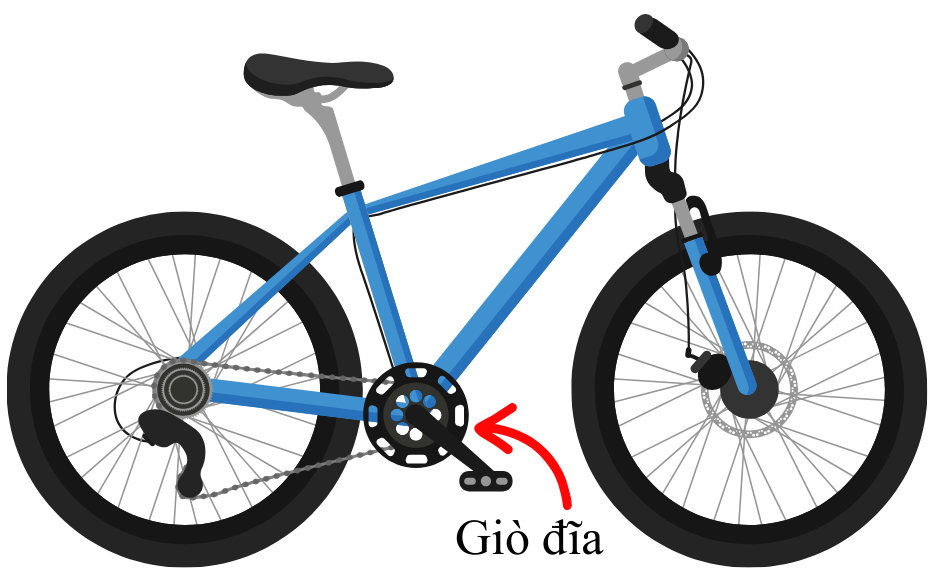
\includegraphics[height=4cm]{hinh/De6-1.png}
}
\loigiai{
a) $C\approx 2024$ (mm) \hspace{2cm} b) $10\cdot 3\cdot 650\pi=19500\pi\,(\text{mm})\approx61\,(\text{m})$
}
\end{bt}

%%Bài 6:
\begin{bt}[3,0 điểm]
Cho đường tròn $(O;R)$ đường kính $AB$. Kẻ tiếp tuyến $Ax$, lấy $P$ trên $Ax$ ($AP>R$). Từ $P$ kẻ tiếp tuyến $PM$ với $(O)$ ($M$ là tiếp điểm). 
\begin{enumerate}
    \item Chứng minh rằng bốn điểm $A, P, M, O$ cùng thuộc một đường tròn và $BM \parallel OP$.
    \item Đường thẳng vuông góc với $AB$ tại $O$ cắt tia $BM$ tại $N$. Chứng minh tứ giác $OBNP$ là hình bình hành.
    \item Giả sử $AN$ cắt $OP$ tại $K$; $PM$ cắt $ON$ tại $I$; $PN$ cắt $OM$ tại $J$. Chứng minh $I, J, K$ thẳng hàng.
\end{enumerate}
\loigiai{ 
\immini{
\begin{enumerate}
    \item $A,P,O,M$ cùng nằm trên đường tròn đường kính $OP$
    
    Ta có $OP\perp AM, BM\perp AM$ suy ra $OP\parallel BM$.
    \item $\triangle AOP = \triangle OBN \Rightarrow OP = BN$
    
    Ta lại có $BN \parallel OP$ nên $OBNP$ là hình bình hành.

    \item Chứng minh  $I$ là trực tâm $\triangle POJ$ suy ra $IJ \perp OP$ (1)

    Chứng minh $K$ là trung điểm $OP$.

    Lại có: $\widehat{APO} = \widehat{OPI} = \widehat{IOP}$
    
    Suy ra $\triangle IPO$ cân tại $I$ suy ra $IK \perp OP$ (2)

    Từ (1) và (2) suy ra $I, J, K$ thẳng hàng.
\end{enumerate}
}
{
	\begin{tikzpicture}[scale=1, font=\footnotesize, line join =round, line cap=round, >=stealth]
		\def\r{1.8}
		\path 
		(0,0) coordinate (O)
		(180:\r) coordinate (A)
		(0:\r) coordinate (B)
		(-\r,2.5*\r) coordinate (x)node[left]{$x$}
		($(A)!4/5!(x)$) coordinate (P)
		($(O)!(A)!(P)$) coordinate (H)
		($(A)!2!(H)$) coordinate (M)
		($(O)!1cm!-90:(A)$) coordinate (n')
		(intersection of B--M and O--n') coordinate (N)
		(intersection of A--N and O--P) coordinate (K)
		(intersection of O--N and M--P) coordinate (I)
		(intersection of O--M and N--P) coordinate (J)
		;
		\draw 
		(O) circle (\r) 
		(x)--(A)--(B)--(N)--(A)--(M)--(P)--(O)--(N) (P)--(J)--(O)
		;
		\draw[dashed] (K)--(J);
		\foreach \x/\g in{O/-90,A/180,B/0,P/180,K/160,M/0,N/90,I/120,J/40}
		\draw[fill=white] (\x) circle (1.5pt) +(\g:.3) node{$\x$};
	\end{tikzpicture}
}
}
\end{bt}
\Closesolutionfile{ansbook}

	    
	    \newpage %ĐỀ SỐ 7
	    \section{Đề 7}
		\setcounter{ex}{0} %Ba Đồn-Quảng Bình
\subsection{Trắc nghiệm (2 điểm)}
\Opensolutionfile{ans}[ans/ans7]


%%Câu 1:
\begin{ex}
Tìm giá trị của tham số $m$ để hệ phương trình
$\begin{cases}
2x-3y=5\\
(m+1)x-6y=m+3
\end{cases}$
vô nghiệm.
\vspace{0.35cm}
\choice
{\True $m=3$}
{$m=-1$}
{$m=0$}
{$m=5$}
\end{ex}

%%Câu 2:
\begin{ex}
Tổng các nghiệm của phương trình $\dfrac{1}{x+3}+\dfrac{2}{x-3}=\dfrac{x^2+3}{x^2-9}$ bằng
\vspace{0.35cm}
\choice
{$3$}
{$2$}
{$4$}
{\True $0$}
\end{ex}

%%Câu 3:
\begin{ex}
Cho hai đường tròn đồng tâm có bán kính lần lượt là $9\,\text{cm}$ và $6\,\text{cm}$. Phần hình vành khuyên nằm trong một góc ở tâm $120^\circ$ có diện tích bằng
\choice
{$20\pi\,\text{cm}^2$}
{$45\pi\,\text{cm}^2$}
{$30\pi\,\text{cm}^2$}
{\True $15\pi\,\text{cm}^2$}
\end{ex}

%%Câu 4:
\begin{ex}
Tính tổng các giá trị nguyên $x$ thỏa mãn cả hai bất phương trình
$\begin{cases}
2x+1<4x+5\\
3x-1<\dfrac{x}{2}+4
\end{cases}$.
\choice
{$4$}
{$2$}
{\True $0$}
{$1$}
\end{ex}

%%Câu 5:
\begin{ex}
Cho biểu thức
$A=\sqrt{(2x-3)^2}-\sqrt{(x+1)^2}$.
Rút gọn biểu thức $A$ với $-1\le x<\dfrac{3}{2}$, ta được
\choice
{$4-x$}
{\True $2-3x$}
{$2+x$}
{$3x-2$}
\end{ex}

%%Câu 6:
\begin{ex}
Cho tam giác $ABC$ vuông tại $A$, đường cao $AH$ và $AB=30$, $BH=18$. Chu vi tam giác $ABC$ là
\choice
{\True $120$}
{$130$}
{$125$}
{$110$}
\end{ex}

%%Câu 7:
\begin{ex}
Cho hai đường tròn $(O;9\,\text{cm})$ và $(O';4\,\text{cm})$ có $OO'=5\,\text{cm}$. Khẳng định nào sau đây đúng về vị trí tương đối của hai đường tròn?
\choice
{\True Hai đường tròn tiếp xúc trong}
{Hai đường tròn tiếp xúc ngoài}
{Hai đường tròn cắt nhau tại hai điểm}
{Hai đường tròn ở ngoài nhau}
\end{ex}

%%Câu 8:
\begin{ex}
Phương trình $5x(-10x-2)=90x+18$ tương đung với phương trình nào sau đây?
\choice
{$(-10x-2)(5x+10)=0$}
{$(1-10x)(5x+9)=0$}
{\True $(-10x-2)(5x+9)=0$}
{$(2-10x)(5x+9)=0$}
\end{ex}

%%Câu 9:
\begin{ex}
Cho đường tròn $(O;12\,\text{cm})$. Một cung nhỏ của đường tròn có số đo $135^\circ$. Độ dài của cung nhỏ đó bằng
\choice
{$6\pi\,\text{cm}$}
{$12\pi\,\text{cm}$}
{$18\pi\,\text{cm}$}
{\True $9\pi\,\text{cm}$}
\end{ex}

%%Câu 10:
\begin{ex}
Cho đường tròn $(O;5\,\text{cm})$ và điểm $P$ nằm ngoài đường tròn sao cho $OP=13\,\text{cm}$. Từ $P$ kẻ tiếp tuyến $PA$ với đường tròn $(O)$ ($A$ là tiếp điểm). Độ dài đoạn thẳng $PA$ bằng
\choice
{$\sqrt{194}\,\text{cm}$}
{\True $12\,\text{cm}$}
{$8\,\text{cm}$}
{$18\,\text{cm}$}
\end{ex}


\Closesolutionfile{ans}
\Opensolutionfile{ansbook}[ans/ansbook7]
\setcounter{bt}{0}
\subsection{Tự luận (8 điểm)}

%Bài 1:
\begin{bt}[1,5 điểm]
Giải các phương trình, bất phương trình và hệ phương trình sau:
\begin{listEX}[3]
\item $(3x-2)^2-(x+4)^2=0$
\item $\dfrac{3x-2}{4}-\dfrac{x+5}{3}<\dfrac{5x+1}{6}$
\item $\begin{cases}
\dfrac{2x-y}{3}+\dfrac{x+2y}{2}=\dfrac{5}{3}\\
3(x-1)-2(y+2)=1
\end{cases}$
\end{listEX}
\loigiai{
\begin{enumerate}
\item Ta có
\begin{align*}
(3x-2)^2-(x+4)^2&=0\\
\big[(3x-2)-(x+4)\big]\big[(3x-2)+(x+4)\big]&=0\\
(2x-6)(4x+2)&=0.
\end{align*}
Do đó $x=3$ hoặc $x=-\dfrac{1}{2}$.

\item Nhân cả hai vế với $12>0$, ta được
\begin{align*}
3(3x-2)-4(x+5)&<2(5x+1)\\
5x-26&<10x+2\\
-28&<5x\\
x&>-\dfrac{28}{5}.
\end{align*}
Vậy bất phương trình có nghiệm $x>-\dfrac{28}{5}$.

\item Dùng phương pháp cộng đại số, ta có
\begin{align*}
&\begin{cases}
\dfrac{2x-y}{3}+\dfrac{x+2y}{2}=\dfrac{5}{3},\\
3(x-1)-2(y+2)=1
\end{cases}\\[0.7em]
\Leftrightarrow\quad
&\begin{cases}
7x+4y=10,\\
3x-2y=8
\end{cases}\\[0.7em]
\Leftrightarrow\quad
&\begin{cases}
7x+4y=10,\\
6x-4y=16
\end{cases}\\[0.7em]
\Leftrightarrow\quad
&\begin{cases}
13x=26,\\
3x-2y=8
\end{cases}\\[0.7em]
\Leftrightarrow\quad
&\begin{cases}
x=2,\\
y=-1.
\end{cases}
\end{align*}
Vậy hệ phương trình có nghiệm $(x;y)=(2;-1)$.
\end{enumerate}
}
\end{bt}


%Bài 2

\begin{bt}[1 điểm]
Rút gọn các biểu thức sau:
\begin{listEX}[2]
\item $\sqrt{23+8\sqrt{7}}+\sqrt{23-8\sqrt{7}}-\sqrt{14-4\sqrt{10}}$
\item $\dfrac{\sqrt{80}-\sqrt{5}}{\sqrt{5}-\sqrt{3}}+\dfrac{3\sqrt{3}}{\sqrt{5}+\sqrt{3}}$
\end{listEX}
\loigiai{
\begin{enumerate}
\setlength{\itemsep}{1em}

\item Ta có
\begin{align*}
23+8\sqrt{7}
&=16+2\cdot4\sqrt{7}+7\\
&=\left(4+\sqrt{7}\right)^2,\\
23-8\sqrt{7}
&=16-2\cdot4\sqrt{7}+7\\
&=\left(4-\sqrt{7}\right)^2,\\
14-4\sqrt{10}
&=10-2\cdot\sqrt{10}\cdot2+4\\
&=\left(\sqrt{10}-2\right)^2.
\end{align*}
Vì $4-\sqrt{7}>0$ và $\sqrt{10}-2>0$ nên
\begin{align*}
\sqrt{23+8\sqrt{7}}+\sqrt{23-8\sqrt{7}}
-\sqrt{14-4\sqrt{10}}\\
&=4+\sqrt{7}+4-\sqrt{7}-\left(\sqrt{10}-2\right)\\
&=10-\sqrt{10}.
\end{align*}
Vậy biểu thức đã cho rút gọn thành $10-\sqrt{10}$.

\item Ta có $\sqrt{80}=4\sqrt{5}$, do đó
\begin{align*}
\dfrac{\sqrt{80}-\sqrt{5}}{\sqrt{5}-\sqrt{3}}
+\dfrac{3\sqrt{3}}{\sqrt{5}+\sqrt{3}}\\
&=\dfrac{3\sqrt{5}}{\sqrt{5}-\sqrt{3}}
+\dfrac{3\sqrt{3}}{\sqrt{5}+\sqrt{3}}\\
&=\dfrac{3\sqrt{5}\left(\sqrt{5}+\sqrt{3}\right)}{5-3}
+\dfrac{3\sqrt{3}\left(\sqrt{5}-\sqrt{3}\right)}{5-3}\\
&=\dfrac{15+3\sqrt{15}+3\sqrt{15}-9}{2}\\
&=3+3\sqrt{15}.
\end{align*}
Vậy biểu thức đã cho rút gọn thành $3+3\sqrt{15}$.
\end{enumerate}
}
\end{bt}

%Bài 3
\begin{bt}[1,0 điểm]
Cô Hà mua dụng cụ học tập tại một cửa hàng. Lần thứ nhất, cô mua $5$ cây bút và $3$ quyển vở hết $70\,000$ đồng. Lần thứ hai, cô mua $2$ cây bút và $4$ quyển vở hết $56\,000$ đồng. Biết các cây bút cùng giá và các quyển vở cùng giá. Tính giá tiền của một cây bút và một quyển vở.
\loigiai{
Gọi $x$ (nghìn đồng) là giá một cây bút và $y$ (nghìn đồng) là giá một quyển vở, với $x>0$, $y>0$.

Lần mua thứ nhất cho ta
\[
5x+3y=70. \tag{1}
\]
Lần mua thứ hai cho ta
\[
2x+4y=56. \tag{2}
\]
Chia hai vế của $(2)$ cho $2$:
\[
x+2y=28 \Rightarrow x=28-2y. \tag{3}
\]
Thế $(3)$ vào $(1)$:
\begin{align*}
5(28-2y)+3y&=70\\
140-10y+3y&=70\\
140-7y&=70\\
-7y&=-70\\
y&=10.
\end{align*}
Thay $y=10$ vào $(3)$:
\[
x=28-2\cdot 10=8.
\]
Cặp $(x;y)=(8;10)$ thỏa $x>0$, $y>0$.

\emph{Kiểm tra.}
\(5\cdot 8+3\cdot 10=70\) và \(2\cdot 8+4\cdot 10=56\), đúng với giả thiết.

Vậy một cây bút giá $8\,000$ đồng và một quyển vở giá $10\,000$ đồng.
}
\end{bt}

%Bài 4

\begin{bt}[1,0 điểm]
	Tính chiều cao $CD$ của một ngọn núi, biết tại hai điểm $A$ và $B$ cách nhau $1$ km trên mặt đất, người ta nhìn thấy đỉnh núi $D$ với góc nâng lần lượt là $30^\circ$ và $45^\circ$ (làm tròn đến hai chữ số thập phân sau dấu phẩy).
	\begin{center}
		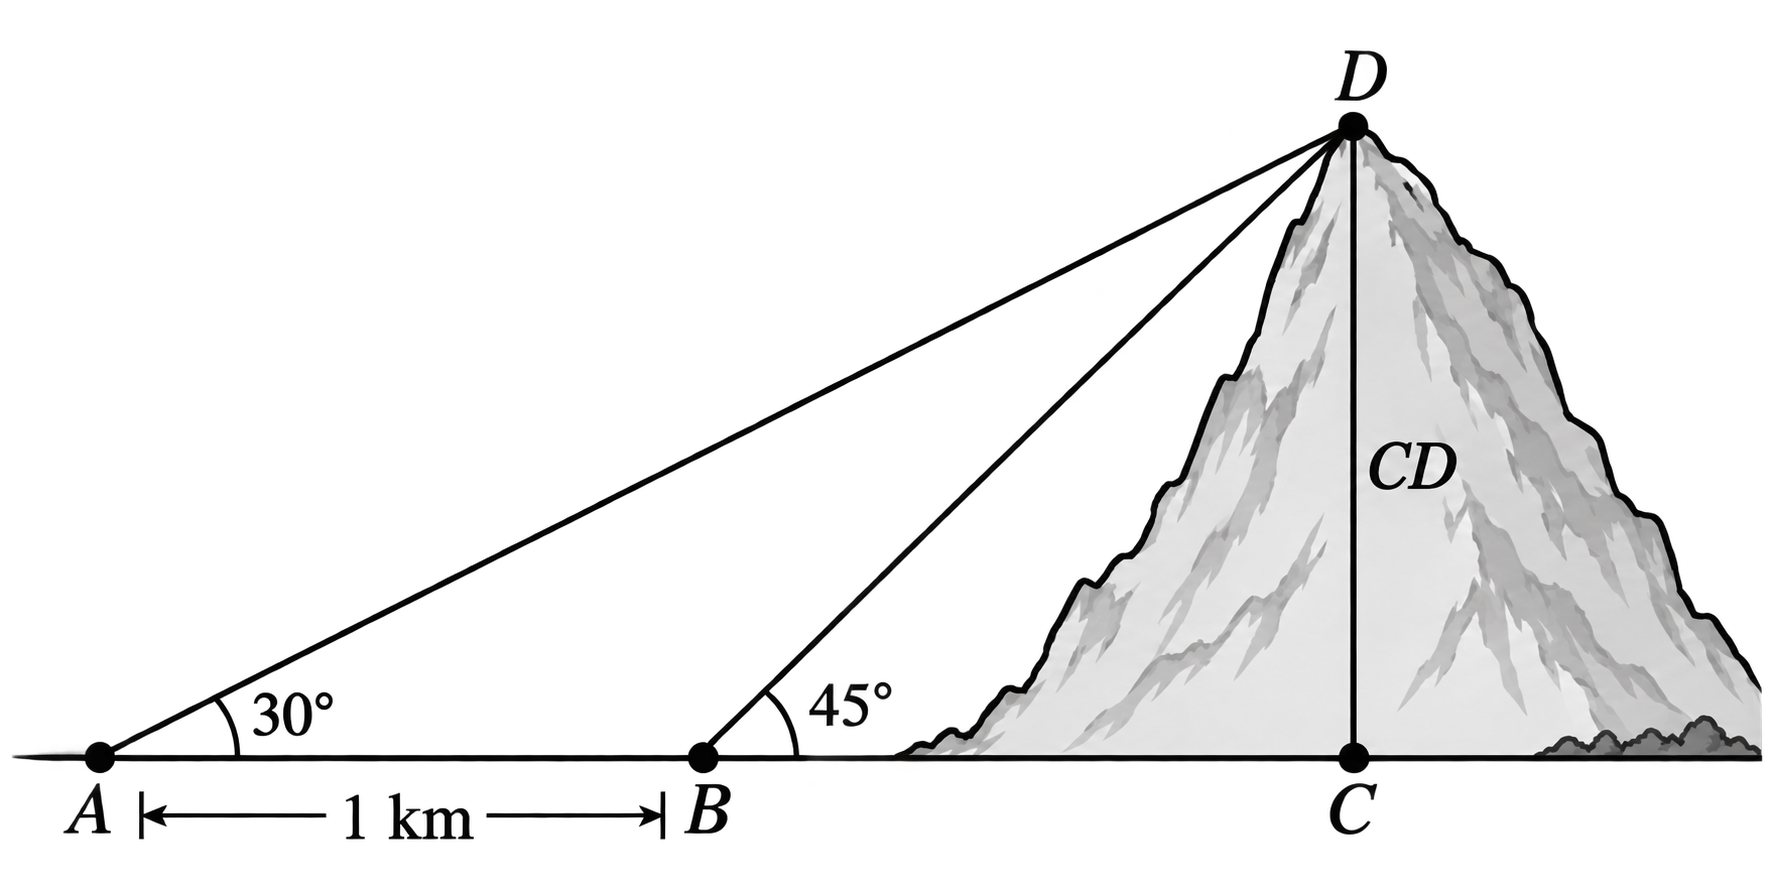
\includegraphics[width=0.45\textwidth]{hinh/De7-cau4.png}
	\end{center}
	
	\loigiai{
	Đổi $1$ km $=1000$ m.
	
	Xét tam giác $DCB$ vuông tại $C$, ta có:
	\[
	\tan\widehat{DBC}=\dfrac{DC}{BC}
	\Rightarrow BC=\dfrac{DC}{\tan45^\circ}.
	\]
	
	Xét tam giác $DCA$ vuông tại $C$, ta có:
	\[
	\tan\widehat{DAC}=\dfrac{DC}{AC}
	\Rightarrow AC=\dfrac{DC}{\tan30^\circ}.
	\]
	
	Ta có:
	\[
	AC-BC=AB
	\Rightarrow
	\dfrac{DC}{\tan30^\circ}
	-\dfrac{DC}{\tan45^\circ}
	=1000.
	\]
	
	Suy ra:
	\[
	DC\left(
	\dfrac{1}{\tan30^\circ}
	-\dfrac{1}{\tan45^\circ}
	\right)=1000.
	\]
	
	Vậy chiều cao của ngọn núi là
	\[
	DC=1000:
	\left(
	\dfrac{1}{\tan30^\circ}
	-\dfrac{1}{\tan45^\circ}
	\right)
	\approx 1366{,}03\text{ (m)}.
	\]
	}
\end{bt}
	

%Câu 5
\begin{bt}[1,0 điểm]
\immini[thm]
{Một tấm gỗ hình tròn bán kính $16$ cm được gắn chính giữa một gương tròn bán kính $10$ cm. Phần gỗ còn nhìn thấy là một hình vành khuyên (hình vẽ). Lấy $\pi=3{,}14$.
\begin{enumerate}
\item Tính diện tích phần gỗ còn nhìn thấy (làm tròn kết quả đến hàng phần mười centimét vuông).
\item Người ta dán một đường kim tuyến quanh mép ngoài của tấm gỗ. Tính độ dài đường kim tuyến đó (làm tròn kết quả đến hàng phần mười centimét).
\end{enumerate}
}
{
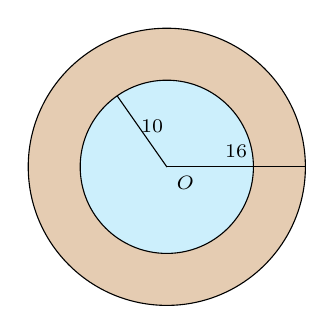
\begin{tikzpicture}[scale=0.11, font=\scriptsize, line join=round]
	\fill[brown!40] (0,0) circle (16);
	\fill[cyan!20] (0,0) circle (10);
	\draw (0,0) circle (16);
	\draw (0,0) circle (10);
	\draw (0,0)--(16,0);
	\node[above] at (8,0) {$16$};
	\draw (0,0)--(125:10);
	\node[above right] at (145:5) {$10$};
	\fill (0,0) circle (2pt) node[below right] {$O$};
\end{tikzpicture}
}
\loigiai{
\begin{enumerate}
\item Phần gỗ còn nhìn thấy là hình vành khuyên có bán kính ngoài $R=16$ cm và bán kính trong $r=10$ cm. Diện tích phần này là
\begin{align*}
S&=\pi R^2-\pi r^2\\
&=\pi\left(16^2-10^2\right)\\
&=3{,}14(256-100)\\
&=3{,}14\cdot 156\\
&=489{,}84\ \text{(cm}^2\text{)}.
\end{align*}
Làm tròn đến hàng phần mười: $S\approx 489{,}8$ cm$^2$.

Vậy diện tích phần gỗ còn nhìn thấy khoảng $489{,}8$ cm$^2$.

\item Đường kim tuyến là chu vi đường tròn mép ngoài, bán kính $16$ cm:
\begin{align*}
C&=2\pi R\\
&=2\cdot 3{,}14\cdot 16\\
&=100{,}48\ \text{(cm)}.
\end{align*}
Làm tròn đến hàng phần mười: $C\approx 100{,}5$ cm.

Vậy độ dài đường kim tuyến khoảng $100{,}5$ cm.
\end{enumerate}
}
\end{bt}

%Bài 6
\begin{bt}[2,5 điểm]
Cho nửa đường tròn $(O)$, đường kính $AB=2R$. Trên nửa đường tròn lấy điểm $C$ bất kì ($C$ khác $A$ và $B$). Tiếp tuyến tại $C$ và tiếp tuyến tại $A$ cắt nhau tại $M$.
\begin{enumerate}
\item Chứng minh bốn điểm $O$, $M$, $A$, $C$ cùng thuộc một đường tròn.
\item $AC$ cắt $OM$ tại $H$. Chứng minh $AC\perp OM$ và $OH\cdot OM=R^2$.
\item Tia $BH$ cắt nửa đường tròn tại $D$, tia $AD$ cắt $MH$ tại $I$. Chứng minh $\triangle ODM\backsim\triangle OHD$ và $I$ là trung điểm của $MH$.
\end{enumerate}
\loigiai{
\begin{center}
\begin{tikzpicture}[scale=1.02, font=\footnotesize, line join=round, line cap=round]
	\def\r{2}
	\def\ang{50}
	\pgfmathsetmacro{\hx}{-\r*sin(\ang/2)*sin(\ang/2)}
	\pgfmathsetmacro{\hy}{\r*sin(\ang)/2}
	\coordinate (O) at (0,0);
	\coordinate (A) at (-\r,0);
	\coordinate (B) at (\r,0);
	\coordinate (C) at (\ang:\r);
	\coordinate (M) at (-\r,{\r*cot(\ang/2)});
	\coordinate (H) at (\hx,\hy);
	\pgfmathsetmacro{\dx}{\hx-\r}
	\pgfmathsetmacro{\dy}{\hy}
	\pgfmathsetmacro{\tt}{-2*\r*\dx/(\dx*\dx+\dy*\dy)}
	\coordinate (D) at ({\r+\tt*\dx},{\tt*\dy});
	\path[name path=tiaAD] (A) -- ($(A)!2.6!(D)$);
	\path[name path=doanMH] (M) -- (H);
	\path[name intersections={of=tiaAD and doanMH, by=I}];
	\fill[mauChuDao!8] (A) arc (180:0:\r) -- cycle;
	\draw[thick] (A) arc (180:0:\r);
	\draw[thick] (A)--(B);
	\draw[thick] (M)--(A) (M)--(C);
	\draw (A)--(C) (O)--(M) (B)--(D) (A)--(I);
	\draw[dashed] (O)--(C);
	\draw ($(A)+(0.2,0)$)--++(0,0.2)--++(-0.2,0);
	\pic[draw, angle radius=0.18cm] {right angle=A--H--M};
	\foreach \p/\pos in {O/below, A/below left, B/below right, C/above right, M/left}
		\fill (\p) circle (1.15pt) node[\pos] {$\p$};
	\fill (D) circle (1.15pt) node[left=2pt] {$D$};
	\fill (H) circle (1.15pt) node[below left=1pt, fill=white, inner sep=1.1pt] {$H$};
	\fill (I) circle (1.15pt) node[right=2pt, fill=white, inner sep=1.1pt] {$I$};
\end{tikzpicture}
\end{center}
\begin{enumerate}
\setlength{\itemsep}{0.8em}
\item Vì tiếp tuyến tại $A$ vuông góc với bán kính qua tiếp điểm nên $OA\perp MA$, tức là $\widehat{OAM}=90^\circ$.
Vì tiếp tuyến tại $C$ vuông góc với bán kính qua tiếp điểm nên $OC\perp MC$, tức là $\widehat{OCM}=90^\circ$.

Tam giác $OAM$ vuông tại $A$ và có cạnh huyền $OM$, nên $A$ thuộc đường tròn đường kính $OM$.
Tam giác $OCM$ vuông tại $C$ và có cạnh huyền $OM$, nên $C$ thuộc đường tròn đường kính $OM$.
Hai điểm $O$ và $M$ cũng thuộc đường tròn đường kính $OM$.

Vậy bốn điểm $O$, $M$, $A$, $C$ cùng thuộc một đường tròn, đó là đường tròn đường kính $OM$.

\item Hai tiếp tuyến xuất phát từ $M$ thì bằng nhau, nên $MA=MC$.

Xét $\triangle OAM$ và $\triangle OCM$:
\[
OA=OC,\qquad MA=MC,\qquad OM\text{ chung}.
\]
Suy ra $\triangle OAM\cong\triangle OCM$ (c.c.c), nên $\widehat{AMO}=\widehat{CMO}$.

Hai tam giác này nằm hai bên đường thẳng $OM$, nên tia phân giác của $\widehat{AMC}$ xuất phát từ $M$, đi trên đường thẳng $OM$ và cắt $AC$ tại $H$. Do đó $\widehat{AMH}=\widehat{CMH}$.

Xét $\triangle AMH$ và $\triangle CMH$:
\[
MA=MC,\qquad \widehat{AMH}=\widehat{CMH},\qquad MH\text{ chung}.
\]
Suy ra $\triangle AMH\cong\triangle CMH$ (c.g.c), nên $\widehat{AHM}=\widehat{CHM}$ và $AH=CH$.

Hai góc $\widehat{AHM}$ và $\widehat{CHM}$ kề nhau và có tổng bằng $180^\circ$ vì $A$, $H$, $C$ thẳng hàng. Hai góc bằng nhau nên
\[
\widehat{AHM}=\widehat{CHM}=90^\circ.
\]
Vậy $AC\perp OM$. Đồng thời $H$ là trung điểm của $AC$.

Trong tam giác $OAM$ vuông tại $A$, các góc ở $O$ và ở $M$ đều nhọn, nên chân đường vuông góc kẻ từ $A$ xuống cạnh huyền $OM$ nằm giữa $O$ và $M$. Chân đường vuông góc đó chính là $H$, vì $AH\perp OM$ và $H$ nằm trên $OM$.

Theo hệ thức lượng trong tam giác vuông $OAM$,
\[
OA^2=OH\cdot OM.
\]
Mà $OA=R$, nên $OH\cdot OM=R^2$.

\item Tia $BH$ cắt nửa đường tròn tại $D$, nên $D$ thuộc đường tròn $(O)$ và $OD=R$.
Theo câu b),
\[
OH\cdot OM=R^2=OD^2,
\]
do đó
\[
\dfrac{OD}{OH}=\dfrac{OM}{OD}.
\]
Vì $H$ nằm trên tia $OM$ nên $\widehat{DOM}$ và $\widehat{HOD}$ là cùng một góc.

Xét $\triangle ODM$ và $\triangle OHD$: góc ở $O$ chung, hai cạnh kề góc này tỉ lệ theo đẳng thức trên. Cụ thể, cạnh $OD$ của $\triangle ODM$ ứng với cạnh $OH$ của $\triangle OHD$, cạnh $OM$ ứng với cạnh $OD$. Suy ra
\[
\triangle ODM\backsim\triangle OHD
\quad\text{(c.g.c)}.
\]

Chứng minh $I$ là trung điểm của $MH$.

Vì $AB$ là đường kính và $D$ thuộc nửa đường tròn nên $\widehat{ADB}=90^\circ$. Do đó $AD\perp BD$. Mà $H$ nằm trên $BD$, nên đường thẳng $AD$ vuông góc với đường thẳng $BH$.

Chọn hệ trục tọa độ có gốc tại $H$, tia hoành dương hướng từ $H$ đến $M$ và tia tung dương hướng từ $H$ đến $A$. Hệ trục này vuông góc vì $AC\perp OM$.

Đặt $OH=h$, $HM=m$ và $AH=a$, với $h,m,a>0$. Khi đó
\[
H=(0;0),\qquad M=(m;0),\qquad A=(0;a).
\]
Vì $H$ nằm giữa $O$ và $M$ nên $O=(-h;0)$.

Trong tam giác vuông $OAM$, đường cao $AH$ cho hệ thức $AH^2=OH\cdot HM$, nên $a^2=hm$.
Lại có $OA^2=OH^2+AH^2$, nên
\[
R^2=h^2+a^2.
\]

Vì $O$ là trung điểm của $AB$ nên tọa độ $O$ là trung bình cộng tọa độ của $A$ và $B$. Gọi $B=(x_B;y_B)$, ta có
\[
\dfrac{0+x_B}{2}=-h,\qquad \dfrac{a+y_B}{2}=0.
\]
Suy ra $B=(-2h;-a)$.

Đường thẳng $BH$ đi qua $H=(0;0)$ và $B=(-2h;-a)$, nên có phương trình tham số
\[
\begin{cases}
x=-2hs,\\
y=-as,
\end{cases}
\quad s\in\mathbb{R}.
\]
Điểm $B$ ứng với $s=1$. Tia $BH$ đi từ $B$ qua $H$ rồi cắt đường tròn lần nữa tại $D$, nên $D$ ứng với giá trị $s<0$.

Vì $D$ thuộc đường tròn tâm $O=(-h;0)$, bán kính $R$, nên
\begin{align*}
(-2hs+h)^2+(-as)^2&=R^2\\
h^2(1-2s)^2+a^2s^2&=h^2+a^2\\
h^2(1-4s+4s^2)+a^2s^2&=h^2+a^2\\
(4h^2+a^2)s^2-4h^2s-a^2&=0.
\end{align*}
Thay $s=1$ thỏa mãn phương trình, nên $s-1$ là một nhân tử. Phân tích, ta được
\[
(s-1)\bigl[(4h^2+a^2)s+a^2\bigr]=0.
\]
Suy ra $s=1$ hoặc
\[
s=-\dfrac{a^2}{4h^2+a^2}.
\]
Giá trị $s=1$ cho điểm $B$. Điểm $D$ ứng với
\[
s=-\dfrac{a^2}{4h^2+a^2}=-\dfrac{hm}{4h^2+hm}=-\dfrac{m}{4h+m}.
\]
Do đó
\begin{align*}
x_D&=-2h\left(-\dfrac{m}{4h+m}\right)=\dfrac{2hm}{4h+m},\\
y_D&=-a\left(-\dfrac{m}{4h+m}\right)=\dfrac{am}{4h+m}.
\end{align*}

Đường thẳng $AD$ đi qua $A=(0;a)$ và $D$. Một điểm trên $AD$ có dạng
\[
(1-u)A+uD
=\left(
\dfrac{2hmu}{4h+m};\;
(1-u)a+\dfrac{amu}{4h+m}
\right),\quad u\in\mathbb{R}.
\]
Điểm $I=AD\cap MH$ nằm trên trục hoành, nên tung độ bằng $0$:
\begin{align*}
(1-u)a+\dfrac{amu}{4h+m}&=0\\
1-u+\dfrac{mu}{4h+m}&=0\\
1&=u\left(1-\dfrac{m}{4h+m}\right)
=u\cdot\dfrac{4h}{4h+m}.
\end{align*}
Suy ra $u=\dfrac{4h+m}{4h}$. Hoành độ của $I$ là
\[
x_I=\dfrac{4h+m}{4h}\cdot\dfrac{2hm}{4h+m}=\dfrac{m}{2}.
\]
Vậy $I=\left(\dfrac{m}{2};0\right)$, tức là trung điểm của đoạn thẳng $MH$.
\end{enumerate}
}
\end{bt}

\Closesolutionfile{ansbook}

	    
	    \newpage %ĐỀ SỐ 8
	    \section{Đề 8}
		\setcounter{ex}{0} %Thái Hòa-Nghệ An
\subsection{Trắc nghiệm (2 điểm)}
\Opensolutionfile{ans}[ans/ans8]

%%Câu 1:
\begin{ex}
Hai đường thẳng $x+by=6$, $ax+by=12$ cùng đi qua điểm $(3;-3)$. Giá trị của $a$ và $b$ là
\choice
{\True $a=3;b=-1$}
{$a=4;b=-1$}
{$a=4;b=0$}
{$a=3;b=0$}
\end{ex}

%%Câu 2:
\begin{ex}
Giá trị của biểu thức $P=\dfrac{1}{\sqrt{7}-\sqrt{5}}-\dfrac{1}{\sqrt{7}+\sqrt{5}}$ bằng
\choice
{$\sqrt{7}$}
{\True $\sqrt{5}$}
{$2\sqrt{5}$}
{$\sqrt{35}$}
\end{ex}

%%Câu 3:
\begin{ex}
Tính giá trị biểu thức
$F=12\tan32^\circ\tan58^\circ+\sin^251^\circ+\sin^239^\circ-\dfrac{8\cot35^\circ}{\tan55^\circ}$.
\vspace{0.35cm}
\choice
{$3$}
{\True $5$}
{$4$}
{$2$}
\end{ex}

%%Câu 4:
\begin{ex}
Cho hai đường tròn $(O;8\,\text{cm})$ và $(O';3\,\text{cm})$ có $OO'=10\,\text{cm}$. Khẳng định nào sau đây đúng?
\choice
{Hai đường tròn ở ngoài nhau}
{Hai đường tròn tiếp xúc trong}
{\True Hai đường tròn cắt nhau tại hai điểm}
{Hai đường tròn tiếp xúc ngoài}
\end{ex}

%%Câu 5:
\begin{ex}
Cho tam giác $ABC$ vuông tại $A$, đường cao $AH$ có $AB=13\,\text{cm}$; $BH=1{,}1\,\text{dm}$. Tính tỉ số lượng giác $\sin C$ (làm tròn đến chữ số thập phân thứ $2$).
\choice
{$0{,}65$}
{\True $0{,}85$}
{$0{,}95$}
{$0{,}75$}
\end{ex}

%%Câu 6:
\begin{ex}
Một khu du lịch bán hai loại vé tham quan: vé người lớn giá $80\,000$ đồng và vé trẻ em giá $50\,000$ đồng. Trong một buổi sáng, khu du lịch bán được $15$ vé và thu về tổng cộng $960\,000$ đồng. Hỏi khu du lịch đã bán được bao nhiêu vé người lớn?
\choice
{$6$ vé}
{\True $7$ vé}
{$8$ vé}
{$9$ vé}
\end{ex}

%%Câu 7:
\begin{ex}
Điều kiện xác định của căn thức $\sqrt{x+2}$ là
\choice
{$x\le -2$}
{$x\ne -2$}
{\True $x\ge -2$}
{$x>-2$}
\end{ex}

%%Câu 8:
\begin{ex}
Tìm tất cả các giá trị của tham số $m$ để bất phương trình $(m-2)x>m-2$ có tập nghiệm là $x<1$.
\choice
{$m>2$}
{$m=2$}
{\True $m<2$}
{$m\le 2$}
\end{ex}

%%Câu 9:
\begin{ex}
Cho hình quạt tròn có bán kính $6\,\text{cm}$ và độ dài cung tròn tương ứng là $4\pi\,\text{cm}$. Diện tích hình quạt tròn đó bằng
\choice
{$8\pi\,\text{cm}^2$}
{$10\pi\,\text{cm}^2$}
{$16\pi\,\text{cm}^2$}
{\True $12\pi\,\text{cm}^2$}
\end{ex}

%%Câu 10:
\begin{ex}
Cho phương trình $(2m-1)x=m+3$ với $m$ là tham số. Tìm giá trị của $m$ để phương trình vô nghiệm.
\choice
{$m=-3$}
{$m=0$}
{\True $m=\dfrac{1}{2}$}
{$m=3$}
\end{ex}


\Closesolutionfile{ans}
\Opensolutionfile{ansbook}[ans/ansbook8]
\setcounter{bt}{0}
\subsection{Tự luận (8 điểm)}

%Bài 1
\begin{bt}[1,5 điểm]
Giải các phương trình, bất phương trình và hệ phương trình sau:
\begin{listEX}[3]
\item $\dfrac{x+2}{x-1}+\dfrac{x-3}{x+1}=\dfrac{4x+2}{x^2-1}$
\item $\dfrac{2x-3}{3}-\dfrac{x+4}{2}\le\dfrac{5(x-2)}{6}$
\item $\begin{cases}
(x+2)(y-1)=xy-6\\
(x-1)(y+3)=xy+4
\end{cases}$
\end{listEX}
\loigiai{
\begin{enumerate}
\item Điều kiện xác định: $x\ne 1$, $x\ne -1$.
\begin{align*}
\dfrac{x+2}{x-1}+\dfrac{x-3}{x+1}&=\dfrac{4x+2}{x^2-1}\\
(x+2)(x+1)+(x-3)(x-1)&=4x+2\\
2x^2-5x+3&=0\\
(2x-3)(x-1)&=0.
\end{align*}
Suy ra $x=\dfrac{3}{2}$ hoặc $x=1$. \\
Vì $x=1$ không thỏa mãn điều kiện xác định nên phương trình có nghiệm $x=\dfrac{3}{2}$.

\item Nhân cả hai vế với $6>0$, ta được
\begin{align*}
2(2x-3)-3(x+4)&\le 5(x-2)\\
x-18&\le 5x-10\\
-8&\le 4x\\
x&\ge -2.
\end{align*}
Vậy bất phương trình có nghiệm $x\ge -2$.

\item Dùng phương pháp thế, ta có
\begin{align*}
&\begin{cases}
(x+2)(y-1)=xy-6,\\
(x-1)(y+3)=xy+4
\end{cases}\\[0.7em]
\Leftrightarrow\quad
&\begin{cases}
x-2y=4,\\
3x-y=7
\end{cases}\\[0.7em]
\Leftrightarrow\quad
&\begin{cases}
x=4+2y,\\
3x-y=7
\end{cases}\\[0.7em]
\Leftrightarrow\quad
&\begin{cases}
x=4+2y,\\
3(4+2y)-y=7
\end{cases}\\[0.7em]
\Leftrightarrow\quad
&\begin{cases}
x=4+2y,\\
5y=-5
\end{cases}\\[0.7em]
\Leftrightarrow\quad
&\begin{cases}
x=2,\\
y=-1.
\end{cases}
\end{align*}
Vậy hệ phương trình có nghiệm $(x;y)=(2;-1)$.
\end{enumerate}
}
\end{bt}


%Bài 2

\begin{bt}[1 điểm]
Rút gọn các biểu thức sau:
\begin{listEX}[1]
\item $A=\sqrt{x+6\sqrt{x}+9}+\sqrt{x-4\sqrt{x}+4}
-\sqrt{x-10\sqrt{x}+25}$, với $4\le x\le 25$.

\item $B=\left(\dfrac{\sqrt{x}+2}{\sqrt{x}-2}
-\dfrac{\sqrt{x}-2}{\sqrt{x}+2}\right)
\cdot\dfrac{x-4}{8}$, với $x\ge 0,\ x\ne 4$.
\end{listEX}
\loigiai{
\begin{enumerate}
\setlength{\itemsep}{1em}

\item Ta có
\begin{align*}
x+6\sqrt{x}+9&=\left(\sqrt{x}+3\right)^2,\\
x-4\sqrt{x}+4&=\left(\sqrt{x}-2\right)^2,\\
x-10\sqrt{x}+25&=\left(\sqrt{x}-5\right)^2.
\end{align*}
Vì $4\le x\le25$ nên $2\le\sqrt{x}\le5$. Do đó
\begin{align*}
A
&=\left|\sqrt{x}+3\right|
+\left|\sqrt{x}-2\right|
-\left|\sqrt{x}-5\right|\\
&=\sqrt{x}+3+\sqrt{x}-2-\left(5-\sqrt{x}\right)\\
&=3\sqrt{x}-4.
\end{align*}
Vậy $A=3\sqrt{x}-4$.

\item Với $x\ge0$ và $x\ne4$, ta có
\begin{align*}
B
&=\left(\dfrac{\sqrt{x}+2}{\sqrt{x}-2}
-\dfrac{\sqrt{x}-2}{\sqrt{x}+2}\right)
\cdot\dfrac{x-4}{8}\\
&=\dfrac{\left(\sqrt{x}+2\right)^2
-\left(\sqrt{x}-2\right)^2}{x-4}
\cdot\dfrac{x-4}{8}\\
&=\dfrac{8\sqrt{x}}{x-4}\cdot\dfrac{x-4}{8}\\
&=\sqrt{x}.
\end{align*}
Vậy $B=\sqrt{x}$.
\end{enumerate}
}
\end{bt}


%Bài 3
\begin{bt}[1,0 điểm]
Một rạp chiếu phim bán vé người lớn và vé trẻ em. Buổi sáng, rạp bán $3$ vé người lớn và $2$ vé trẻ em, thu được $400\,000$ đồng. Buổi chiều, giá vé người lớn giảm $25\%$ và giá vé trẻ em giảm $10\%$ so với buổi sáng; rạp bán $4$ vé người lớn và $2$ vé trẻ em, thu được $390\,000$ đồng. Biết trong mỗi buổi, các vé cùng loại có cùng giá. Tính giá một vé người lớn và một vé trẻ em ở buổi sáng.
\loigiai{
Gọi $x$ (nghìn đồng) là giá một vé người lớn buổi sáng và $y$ (nghìn đồng) là giá một vé trẻ em buổi sáng, với $x>0$, $y>0$.

Buổi sáng cho ta
\[
3x+2y=400. \tag{1}
\]
Buổi chiều, vé người lớn có giá $\dfrac{3}{4}x$ và vé trẻ em có giá $\dfrac{9}{10}y$, nên
\[
4\cdot\dfrac{3}{4}x+2\cdot\dfrac{9}{10}y=390,
\]
tức là
\[
3x+\dfrac{9}{5}y=390.
\]
Nhân hai vế với $5$:
\[
15x+9y=1950.
\]
Chia hai vế cho $3$:
\[
5x+3y=650. \tag{2}
\]
Nhân $(2)$ với $2$ và nhân $(1)$ với $3$:
\begin{align*}
10x+6y&=1300, \tag{3}\\
9x+6y&=1200. \tag{4}
\end{align*}
Lấy $(3)$ trừ $(4)$:
\[
x=100.
\]
Thay vào $(1)$:
\[
3\cdot 100+2y=400 \Rightarrow 2y=100 \Rightarrow y=50.
\]
Cặp $(x;y)=(100;50)$ thỏa $x>0$, $y>0$.

\emph{Kiểm tra.} Buổi chiều, vé người lớn giá $75$ nghìn đồng và vé trẻ em giá $45$ nghìn đồng.
\[
4\cdot 75+2\cdot 45=300+90=390,
\]
đúng với giả thiết.

Vậy buổi sáng, một vé người lớn giá $100\,000$ đồng và một vé trẻ em giá $50\,000$ đồng.
}
\end{bt}

%Bài 4
\begin{bt}[1,0 điểm]
\immini[thm]
{Một biển hiệu hình chữ nhật có chiều dài $(x+5)$ cm và chiều rộng $(x+1)$ cm, với $x>0$. Ở giữa biển hiệu có một hình tròn bán kính $2$ cm nằm trọn trong hình chữ nhật (hình vẽ). Phần tô đậm là phần hình chữ nhật nằm ngoài hình tròn.
\begin{enumerate}
\item Viết biểu thức diện tích hình chữ nhật, diện tích hình tròn và diện tích phần tô đậm theo $x$.
\item Biết diện tích phần tô đậm là $32-4\pi$ (cm$^2$). Tìm $x$.
\end{enumerate}
}
{
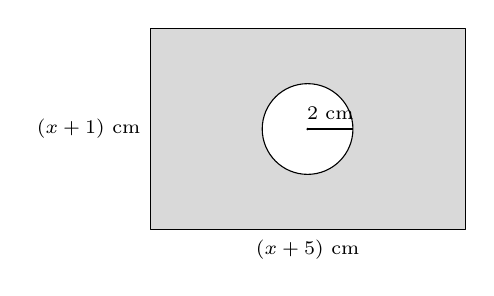
\begin{tikzpicture}[scale=0.8, font=\scriptsize, line join=round]
	\fill[gray!30] (0,0) rectangle (5,3.2);
	\fill[white] (2.5,1.6) circle (0.72);
	\draw (0,0) rectangle (5,3.2);
	\draw (2.5,1.6) circle (0.72);
	\draw (2.5,1.6)--(3.22,1.6);
	\node[above] at (2.86,1.6) {$2$ cm};
	\node[below] at (2.5,0) {$(x+5)$ cm};
	\node[left] at (0,1.6) {$(x+1)$ cm};
	\fill (2.5,1.6) circle (0.6pt);
\end{tikzpicture}
}
\loigiai{
\begin{enumerate}
\item Diện tích hình chữ nhật là
\[
S_{\text{cn}}=(x+5)(x+1)=x^2+6x+5\ \text{(cm}^2\text{)}.
\]
Diện tích hình tròn bán kính $2$ cm là
\[
S_{\text{tròn}}=\pi\cdot 2^2=4\pi\ \text{(cm}^2\text{)}.
\]
Diện tích phần tô đậm là
\[
S=S_{\text{cn}}-S_{\text{tròn}}=x^2+6x+5-4\pi\ \text{(cm}^2\text{)}.
\]

\item Ta có
\begin{align*}
x^2+6x+5-4\pi&=32-4\pi\\
x^2+6x+5&=32\\
x^2+6x-27&=0\\
(x+9)(x-3)&=0.
\end{align*}
Suy ra $x=-9$ hoặc $x=3$.

Vì $x>0$ nên $x=-9$ bị loại. Với $x=3$, hình chữ nhật có chiều dài $8$ cm và chiều rộng $4$ cm. Đường kính hình tròn bằng $4$ cm nên hình tròn tiếp xúc hai cạnh chiều rộng và nằm trọn trong hình chữ nhật.

Vậy $x=3$ cm.
\end{enumerate}
}
\end{bt}

%Bài 5
\begin{bt}[1,0 điểm]
\immini[thm]
{Một đường chạy bộ là hình vành khuyên tâm $O$. Bán kính mép trong là $5$ m và diện tích mặt đường chạy là $75\pi$ (m$^2$). Hai bán kính $OA$, $OB$ của mép ngoài tạo góc $\widehat{AOB}=60^\circ$ (hình vẽ).
\begin{enumerate}
\item Tính bán kính mép ngoài của đường chạy.
\item Tính độ dài cung nhỏ $AB$ và diện tích phần đường chạy nằm trong góc $\widehat{AOB}$.
\end{enumerate}
}
{
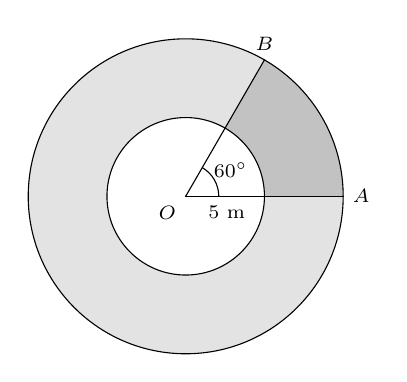
\begin{tikzpicture}[scale=0.2, font=\scriptsize, line join=round]
	\fill[gray!22] (0,0) circle (10);
	\fill[white] (0,0) circle (5);
	\fill[gray!48] (5,0) arc (0:60:5) -- (60:10) arc (60:0:10) -- cycle;
	\draw (0,0) circle (5);
	\draw (0,0) circle (10);
	\draw (0,0)--(10,0);
	\draw (0,0)--(60:10);
	\draw (2.1,0) arc (0:60:2.1);
	\node at (30:3.3) {$60^\circ$};
	\node[below] at (2.6,0) {$5$ m};
	\fill (0,0) circle (1.4pt) node[below left] {$O$};
	\fill (10,0) circle (1.4pt) node[right] {$A$};
	\fill (60:10) circle (1.4pt) node[above] {$B$};
\end{tikzpicture}
}
\loigiai{
\begin{enumerate}
\item Gọi $R$ (m) là bán kính mép ngoài, $R>5$. Diện tích hình vành khuyên là
\begin{align*}
\pi R^2-\pi\cdot 5^2&=75\pi\\
R^2-25&=75\\
R^2&=100.
\end{align*}
Vì $R>0$ nên $R=10$.

Vậy bán kính mép ngoài là $10$ m.

\item Cung nhỏ $AB$ thuộc đường tròn bán kính $10$ m và chắn góc ở tâm $60^\circ$, nên
\[
\ell_{\overset{\frown}{AB}}
=\dfrac{\pi Rn}{180}
=\dfrac{\pi\cdot 10\cdot 60}{180}
=\dfrac{10\pi}{3}\ \text{(m)}.
\]
Phần đường chạy trong góc $\widehat{AOB}$ là hình quạt vành khuyên, bằng hiệu hai hình quạt cùng góc $60^\circ$:
\begin{align*}
S
&=\dfrac{60}{360}\pi\cdot 10^2-\dfrac{60}{360}\pi\cdot 5^2\\
&=\dfrac{1}{6}\pi(100-25)\\
&=\dfrac{75\pi}{6}
=\dfrac{25\pi}{2}\ \text{(m}^2\text{)}.
\end{align*}
Vậy cung nhỏ $AB$ dài $\dfrac{10\pi}{3}$ m và phần đường chạy trong góc $\widehat{AOB}$ có diện tích $\dfrac{25\pi}{2}$ m$^2$.
\end{enumerate}
}
\end{bt}

%Câu 6

\begin{bt}
	Cho nửa đường tròn $(O;R)$ có đường kính $MN$. Kẻ hai tiếp tuyến $Mx$ và $Ny$ của nửa đường tròn $(O)$ ($Mx$, $Ny$ và nửa đường tròn $(O)$ thuộc cùng một phía của đường thẳng $MN$). Lấy điểm $A$ bất kỳ thuộc nửa đường tròn $(O)$ ($AM<AN$). Qua $A$, kẻ tiếp tuyến với nửa đường tròn $(O)$ cắt $Mx$ và $Ny$ lần lượt tại $E$ và $F$.
	
	\begin{listEX}[1]
	\item Chứng minh $4$ điểm $M,E,A,O$ cùng thuộc một đường tròn.
	\item Chứng minh $ME+NF=EF$ và $AE\cdot AF=R^2$.
	\item Gọi $H$ là giao điểm của $MF$ và $NE$, $AH$ cắt $MN$ tại $K$. Chứng minh $AK\perp MN$ và $H$ là trung điểm của $AK$.
	\end{listEX}
\end{bt}
\Closesolutionfile{ansbook}

	
	    \newpage %ĐỀ SỐ 9
	    \section{Đề 9}
		\setcounter{ex}{0} 
\subsection{Trắc nghiệm (2 điểm)}
\Opensolutionfile{ans}[ans/ans9] 


%%Câu 1:
\begin{ex}
Hệ phương trình
$\begin{cases}
7x-3y=11\\
4x+y=9
\end{cases}$
có nghiệm $(x;y)$. Tổng $x+y$ bằng
\vspace{0.2cm}
\choice
{$-2$}
{$2$}
{\True $3$}
{$-3$}
\end{ex}

%%Câu 2:
\begin{ex}
Rút gọn biểu thức
$P=\dfrac{\sqrt{5}+\sqrt{3}}{\sqrt{5}-\sqrt{3}}$
ta được kết quả là
\choice
{$4-\sqrt{15}$}
{\True $4+\sqrt{15}$}
{$8+2\sqrt{15}$}
{$1+\sqrt{15}$}
\end{ex}

%%Câu 3:
\begin{ex}
Giá trị nhỏ nhất của biểu thức $P=4x^2-4xy+2y^2$ bằng
\choice
{\True $0$}
{$1$}
{$2$}
{$3$}
\end{ex}

%%Câu 4:
\begin{ex}
Một cửa hàng bán hai loại vở, loại thứ nhất có giá $12\,000$ đồng/quyển và loại thứ hai có giá $18\,000$ đồng/quyển. Trong một ngày, cửa hàng bán được tổng cộng $25$ quyển vở và thu về $360\,000$ đồng. Hỏi cửa hàng đã bán được bao nhiêu quyển vở loại thứ hai?
\choice
{$8$ quyển}
{\True $10$ quyển}
{$12$ quyển}
{$15$ quyển}
\end{ex}

%%Câu 5:
\begin{ex}
Tìm tham số $m$ để phương trình $x(m+4)-2y=-10$ nhận cặp số $(-1;4)$ là nghiệm.
\choice
{\True $m=-2$}
{$m=-1$}
{$m=-3$}
{$m=-4$}
\end{ex}

%%Câu 6:
\begin{ex}
Cho hai đường tròn $(O;6\,\text{cm})$ và $(O';4\,\text{cm})$ có khoảng cách giữa hai tâm là $OO'=m\,\text{cm}$. Điều kiện của $m$ để hai đường tròn cắt nhau tại hai điểm phân biệt là
\choice
{$2\le m\le 10$}
{$m>10$}
{\True $2<m<10$}
{$m=2$}
\end{ex}

%%Câu 7:
\begin{ex}
Tập nghiệm của bất phương trình
$\dfrac{x-1}{3}-\dfrac{2x+1}{4}\ge -1$
là
\choice
{$x\ge\dfrac{5}{2}$}
{$x<\dfrac{5}{2}$}
{$x\ge-\dfrac{5}{2}$}
{\True $x\le\dfrac{5}{2}$}
\end{ex}

%%Câu 8:
\begin{ex}
Cho tam giác $ABC$ vuông tại $A$. Biết $AB=18\,\text{cm}$, $AC=24\,\text{cm}$. Tính số đo góc $\widehat{ACB}$ (kết quả làm tròn đến độ).
\choice
{\True $37^\circ$}
{$32^\circ$}
{$30^\circ$}
{$34^\circ$}
\end{ex}

%%Câu 9:
\begin{ex}
Cho hình quạt tròn có bán kính $9\,\text{cm}$ và diện tích bằng $27\pi\,\text{cm}^2$. Số đo góc ở tâm của hình quạt tròn đó bằng
\choice
{$60^\circ$}
{$90^\circ$}
{\True $120^\circ$}
{$135^\circ$}
\end{ex}

%%Câu 10:
\begin{ex}
Cho hệ phương trình
$\begin{cases}
2x+y=m\\
x-y=3
\end{cases}$
với $m$ là tham số. Tìm điều kiện của $m$ để hệ phương trình có nghiệm $(x;y)$ thỏa mãn $x>0$ và $y>0$.
\choice
{$m\ge 6$}
{$m<6$}
{$m>3$}
{\True $m>6$}
\end{ex}



\Closesolutionfile{ans}
\Opensolutionfile{ansbook}[ans/ansbook9] 
\setcounter{bt}{0} 
\subsection{Tự luận (8 điểm)}
%Bài 1

\begin{bt}[1,5 điểm]
Giải các phương trình, bất phương trình và hệ phương trình sau:
\begin{listEX}[3]
\item $\dfrac{3x+4}{x-1}-\dfrac{x-2}{x+2}=\dfrac{19x+14}{x^2+x-2}$
\item $-2(3x-5)+\dfrac{5x+1}{2}>\dfrac{3-x}{4}$
\item $\begin{cases}
\dfrac{x+2y}{3}-\dfrac{2x-y}{4}=2\\
3(x-y)+2(2x+y)=-9
\end{cases}$
\end{listEX}
\loigiai{
\begin{enumerate}
\item Điều kiện xác định: $x\ne 1$, $x\ne -2$.
\begin{align*}
\dfrac{3x+4}{x-1}-\dfrac{x-2}{x+2}&=\dfrac{19x+14}{x^2+x-2}\\
(3x+4)(x+2)-(x-2)(x-1)&=19x+14\\
2x^2-6x-8&=0\\
(x-4)(x+1)&=0.
\end{align*}
Suy ra $x=4$ hoặc $x=-1$; cả hai giá trị đều thỏa mãn điều kiện xác định. Vậy $S=\{-1;4\}$.

\item Nhân cả hai vế với $4>0$, ta được
\begin{align*}
-8(3x-5)+2(5x+1)&>3-x\\
-14x+42&>3-x\\
39&>13x\\
x&<3.
\end{align*}
Vậy bất phương trình có nghiệm $x<3$.

\item Dùng phương pháp thế, ta có
\begin{align*}
&\begin{cases}
\dfrac{x+2y}{3}-\dfrac{2x-y}{4}=2,\\
3(x-y)+2(2x+y)=-9
\end{cases}\\[0.7em]
\Leftrightarrow\quad
&\begin{cases}
-2x+11y=24,\\
7x-y=-9
\end{cases}\\[0.7em]
\Leftrightarrow\quad
&\begin{cases}
-2x+11y=24,\\
y=7x+9
\end{cases}\\[0.7em]
\Leftrightarrow\quad
&\begin{cases}
-2x+11(7x+9)=24,\\
y=7x+9
\end{cases}\\[0.7em]
\Leftrightarrow\quad
&\begin{cases}
75x=-75,\\
y=7x+9
\end{cases}\\[0.7em]
\Leftrightarrow\quad
&\begin{cases}
x=-1,\\
y=2.
\end{cases}
\end{align*}
Vậy hệ phương trình có nghiệm $(x;y)=(-1;2)$.
\end{enumerate}
}
\end{bt}


%Bài 2
\begin{bt}[2,0 điểm] $ $
\begin{enumerate}
    \item Cho biểu thức: $\mathrm{Q}=\dfrac{2}{2+\sqrt{x}}+\dfrac{1}{2-\sqrt{x}}+\dfrac{2 \sqrt{x}}{x-4}$
    \begin{enumerate}
        \item[i)] Rút gọn $\mathrm{Q}$
        \item[ii)] Tìm các giá trị nguyên $x$ để $\mathrm{Q}$ nhận giá trị nguyên.
    \end{enumerate}
    \item Giải phương trình: $\dfrac{x-1}{x-5}-\dfrac{4 x}{x+5}=\dfrac{9 x-5}{x^2-25}$
\end{enumerate}
\loigiai{
a) i) Q$=\dfrac{3}{\sqrt{x}+2}$, ii) $x=1$ \hfill b) $x=0$ \hfill
}
\end{bt}

%Bài 3
\begin{bt}[1,0 điểm] $ $
Một người đứng cách một cây xanh một khoảng 30 m. Mắt người đó nhìn lên đỉnh ngọn cây và tạo với phương nằm ngang một góc $20^{\circ}$. Mắt người cách mặt đất 1,6 m. Tính chiểu cao của cây. (Tính chính xác đến dm).
\begin{center}
\begin{tikzpicture}[scale=0.7, font=\small, >=stealth]
\coordinate (N) at (0,0);
\coordinate (M) at (0,1.5); 
\coordinate (A) at (15,0); 
\coordinate (H) at (15,1.5);
\coordinate (B) at (15,7); 
\node[anchor=south west] at (11.5,-0.2) {
\includegraphics[height=5cm]{hinh/De9-tree.png}};
\draw[thick] (N) -- (A);
\node[below] at ($(N)!0.5!(A)$) {30 m};
\draw[dashed, thick] (N) -- (M);
\node[right] at ($(N)!0.5!(M)$) {1,6 m};
\draw[dashed, thick] (M) -- (B);
\draw[dashed] (M) -- (H);
\draw[thick] (A) -- (B);
\draw[thick] (2,1.5) arc[start angle=0, end angle=20, radius=2];
\node at (2.5,1.9) {$20^\circ$};
\foreach \p/\pos in {A/below,B/above right,H/right,M/left,N/below}
      \filldraw[fill=black] (\p) circle(0.5pt) node[\pos] {$\p$};
\node[anchor=south west] at (-0.4,-0.15) {
\includegraphics[height=1cm]{hinh/De9-man.png}};
\end{tikzpicture}
\end{center}
\loigiai{Vận tốc dự định $40 \text{ km/h}$ ; quãng đường AB dài $120 \text{ km}$.}
\end{bt}

%Bài 4
\begin{bt}[3,0 điểm]
Từ điểm $M$ nằm ngoài đường tròn $(O, R)$ kẻ hai tiếp tuyến $MB,\, MC$ ($B, C$ là hai tiếp điểm). $OM$ cắt $BC$ tại $H$.
\begin{listEX}
    \item Giả sử $OM=2R$. Tính $BC$ theo $R$.
    \item Kẻ đường kính $BD$ của $(O)$, $MD$ cắt $(O)$ tại $K$. Chứng minh rằng $MK\cdot MD=MH\cdot MO$.
    \item Chứng minh rằng $HC$ là phân giác của góc $KHD$.
\end{listEX}
\loigiai{\immini{
	\begin{listEX}
		\item $BC=R\sqrt{3}$.
		\item Chứng minh $\triangle MCK \backsim \triangle MDC$ từ đó suy ra $MC^2=MK. MD$.
		
		Mặt khác $MC^2=MO\cdot MH$. Từ đó suy ra điều phải chứng minh.
		\item Chứng minh $\widehat{OHD}=\widehat{ODM}=\widehat{KHM}$ thông qua các tam giác đồng dạng.
		\end{listEX}}
	{
	\begin{tikzpicture}[line width=0.8pt]
		\def\R{2}
		\def\A{6}
		\path 
		(0,0) coordinate (O)
		(\A,0) coordinate (M)
		($(O)!0.5!(M)$) coordinate (I)
		;
		\path[name path=ciro] (O) circle (\R);
		\path[name path=cirom] (I) let \p1=($(I)-(O)$) in circle ({veclen(\x1,\y1)});
		\path[name intersections={of=ciro and cirom, by={B,C}}];
		\coordinate (H) at (intersection of O--M and B--C);
		\coordinate (D) at ($(B)!2!(O)$);
		\path[name path=md] (D)--(M);
		\path[name intersections={of=ciro and md,by={D,K}}];
		\draw (B)--(C) (M)--(D);
		\draw
		(O) circle (\R)
		(B)--(O)--(C) (O)--(M)
		(B)--(M)
		(M)--(C) (O)--(D)--(C)--(K)--(H)--(D)
		;
		\foreach \x/\g in{O/-180,M/0,B/60,C/-60,H/45,D/-90,K/90}
		\draw[fill=white] (\x) circle (1.5pt) +(\g:.35) node{$\x$};
	\end{tikzpicture}
	}
}
\end{bt}

%Bài 5
\begin{bt}[1,0 điểm] Một ô tô đi từ A đến B với vận tốc và thời gian dự định. Nếu người đó tăng vận tốc thêm $20 \mathrm{~km} / \mathrm{h}$ thì đến B sớm hơn dự định 1 giờ Nếu người đó giảm vận tốc $10 \mathrm{~km} / \mathrm{h}$ thì đến B muộn hơn 1 giờ. Tính vận tốc dự định và độ dài quãng đường AB 
\loigiai{
Gọi $x$ (km/h) và $y$ (h) lần lượt là vận tốc và thời gian dự định ($x > 10 ; y > 1$).

Từ giá thiết ta có hệ phương trình:
$\begin{cases}
    (x+20)(y-1)=xy \\
    (x-10)(y+1)=xy
\end{cases} $
    \item Giải hệ PT: $x=40$ (nhận) ; $y=3$ (nhận).}
\end{bt}

\Closesolutionfile{ansbook}

	
	    \newpage %ĐỀ SỐ 10
	    \section{Đề 10}
		\setcounter{ex}{0} 
\subsection{Trắc nghiệm (2 điểm)}
\Opensolutionfile{ans}[ans/ans10] 


%%Câu 1:
\begin{ex}
Cho hệ phương trình
$\begin{cases}
-5x-y=-4\\
-4x-y=-3
\end{cases}$
có nghiệm duy nhất $(x;y)$. Giá trị của biểu thức $-2x^2+3y^2$ là
\choice
{$-9$}
{\True $1$}
{$11$}
{$-4$}
\end{ex}

%%Câu 2:
\begin{ex}
Cho biểu thức
$P=\dfrac{\sqrt{x+4}-2}{x}$ với $x>0$.
Bằng cách trục căn thức ở tử và rút gọn biểu thức $P$, ta được kết quả là
\vspace{0.25cm}
\choice
{$\dfrac{\sqrt{x+4}+2}{x}$}
{$\dfrac{1}{\sqrt{x+4}-2}$}
{\True $\dfrac{1}{\sqrt{x+4}+2}$}
{$\dfrac{1}{\sqrt{x+4}+4}$}
\end{ex}

%%Câu 3:
\begin{ex}
Nếu $a,b$ và $c$ là các số bất kì và $a>b$ thì bất đẳng thức nào sau đây luôn đúng?
\choice
{$ac>bc$}
{$a^2>b^2$}
{$c-a>c-b$}
{\True $a+c>b+c$}
\end{ex}

%%Câu 4:
\begin{ex}
Tập nghiệm của phương trình $\sqrt{2x+3}=x$ là
\choice
{\True $S=\{3\}$}
{$S=\{-1\}$}
{$S=\{-1;3\}$}
{$S=\varnothing$}
\end{ex}

%%Câu 5:
\begin{ex}
Hai hãng taxi có bảng giá như sau:
Hãng A thu phí mở cửa $20\,000$ đồng và $12\,000$ đồng cho mỗi km.
Hãng B thu phí mở cửa $50\,000$ đồng và $8\,000$ đồng cho mỗi km.
Gọi $x$ (km) là quãng đường di chuyển $(x>0)$. Hỏi với điều kiện nào của $x$ thì đi hãng A tiết kiệm hơn hãng B?
\choice
{$x>\dfrac{15}{2}$}
{$x\ge\dfrac{15}{2}$}
{$0<x\le\dfrac{15}{2}$}
{\True $0<x<\dfrac{15}{2}$}
\end{ex}

%%Câu 6:
\begin{ex}
Trong các phương trình sau, phương trình nào là phương trình bậc nhất hai ẩn?
\choice
{$2x^2-y=1$}
{\True $\dfrac{3x}{2}-\dfrac{5}{7}y=1$}
{$\dfrac{5}{3x}-\dfrac{2}{y}=\dfrac{1}{2}$}
{$0x+0y=9$}
\end{ex}

%%Câu 7:
\begin{ex}
Cho hai đường tròn đồng tâm $(O)$ có bán kính lần lượt là $10\,\text{cm}$ và $6\,\text{cm}$. Phần hình vành khuyên nằm trong một góc ở tâm $90^\circ$ có diện tích bằng
\choice
{$25\pi\,\text{cm}^2$}
{$64\pi\,\text{cm}^2$}
{\True $16\pi\,\text{cm}^2$}
{$34\pi\,\text{cm}^2$}
\end{ex}

%%Câu 8:
\begin{ex}
Cho đường tròn $(O)$ và điểm $P$ nằm ngoài đường tròn. Từ $P$ kẻ hai tiếp tuyến $PA$, $PB$ với đường tròn $(O)$ ($A$, $B$ là các tiếp điểm). Biết $\widehat{APB}=70^\circ$. Số đo góc $\widehat{AOB}$ bằng
\choice
{\True $110^\circ$}
{$70^\circ$}
{$140^\circ$}
{$55^\circ$}
\end{ex}

%%Câu 9:
\begin{ex}
Gọi $x$ là số tuổi nam giới. Bất đẳng thức nào biểu diễn điều kiện nam giới phải từ đủ 20 tuổi trở lên để đáp ứng quy định về độ tuổi kết hôn?
\choice
{$x>20$}
{\True $x\ge 20$}
{$x\le 20$}
{$x<20$}
\end{ex}

%%Câu 10:
\begin{ex}
Cho đường tròn $(O;13\,\text{cm})$ có dây cung $AB$ cách tâm $O$ một khoảng bằng $5\,\text{cm}$. Độ dài dây cung $AB$ là
\choice
{$12\,\text{cm}$}
{$\sqrt{194}\,\text{cm}$}
{$26\,\text{cm}$}
{\True $24\,\text{cm}$}
\end{ex}

    
\Closesolutionfile{ans}
\Opensolutionfile{ansbook}[ans/ansbook10]
\setcounter{bt}{0}
\subsection{Tự luận (8 điểm)}

%%Bài 1:

\begin{bt}[1,5 điểm]
Giải các phương trình, bất phương trình và hệ phương trình sau:
\begin{listEX}[3]
\item $(2x-1)^2=9(x-2)^2$
\item $3-\dfrac{2x-5}{4}\le\dfrac{3x+1}{6}-\dfrac{x-2}{3}$
\item $\begin{cases}
\dfrac{3x-y}{4}+\dfrac{x+2y}{3}=\dfrac{1}{6}\\
2(x+1)-3(y-2)=-3
\end{cases}$
\end{listEX}


\loigiai{
\begin{enumerate}
\item Ta có
\begin{align*}
&(2x-1)^2=9(x-2)^2\\
&(2x-1)^2-\big[3(x-2)\big]^2=0\\
&\big[(2x-1)-3(x-2)\big]\big[(2x-1)+3(x-2)\big]=0\\
&(5-x)(5x-7)=0.
\end{align*}
Do đó $x=5$ hoặc $x=\dfrac{7}{5}$.

\item Thu gọn vế phải rồi nhân cả hai vế với $12>0$:
\begin{align*}
3-\dfrac{2x-5}{4}&\le \dfrac{x+5}{6}\\
3(17-2x)&\le 2(x+5)\\
51-6x&\le 2x+10\\
41&\le 8x\\
x&\ge \dfrac{41}{8}.
\end{align*}
Vậy bất phương trình có nghiệm $x\ge\dfrac{41}{8}$.

\item Dùng phương pháp cộng đại số, ta có
\begin{align*}
&\begin{cases}
\dfrac{3x-y}{4}+\dfrac{x+2y}{3}=\dfrac{1}{6},\\
2(x+1)-3(y-2)=-3
\end{cases}\\[0.7em]
\Leftrightarrow\quad
&\begin{cases}
13x+5y=2,\\
2x-3y=-11
\end{cases}\\[0.7em]
\Leftrightarrow\quad
&\begin{cases}
39x+15y=6,\\
10x-15y=-55
\end{cases}\\[0.7em]
\Leftrightarrow\quad
&\begin{cases}
49x=-49,\\
2x-3y=-11
\end{cases}\\[0.7em]
\Leftrightarrow\quad
&\begin{cases}
x=-1,\\
y=3.
\end{cases}
\end{align*}
Vậy hệ phương trình có nghiệm $(x;y)=(-1;3)$.
\end{enumerate}
}
\end{bt}


%%Bài 2:

\begin{bt}[1 điểm]
Rút gọn các biểu thức sau:
\begin{listEX}[1]
\item $A=\sqrt{9x^2-12x+4}+\sqrt{4x^2-20x+25}
-\sqrt{x^2-2x+1}$, với $1\le x\le 2$.

\item $B=\left(\dfrac{2}{\sqrt{x}-1}
-\dfrac{3}{\sqrt{x}+1}\right)
\cdot\dfrac{x-1}{\sqrt{x}+5}$,
với $x\ge 0,\ x\ne 1$.
\end{listEX}
\loigiai{
\begin{enumerate}
\setlength{\itemsep}{1em}

\item Ta có
\begin{align*}
9x^2-12x+4&=(3x-2)^2,\\
4x^2-20x+25&=(2x-5)^2,\\
x^2-2x+1&=(x-1)^2.
\end{align*}
Vì $1\le x\le2$ nên $3x-2>0$, $2x-5<0$ và $x-1\ge0$. Do đó
\begin{align*}
A
&=|3x-2|+|2x-5|-|x-1|\\
&=3x-2+5-2x-(x-1)\\
&=4.
\end{align*}
Vậy $A=4$.

\item Với $x\ge0$ và $x\ne1$, ta có
\begin{align*}
B
&=\left(\dfrac{2}{\sqrt{x}-1}
-\dfrac{3}{\sqrt{x}+1}\right)
\cdot\dfrac{x-1}{\sqrt{x}+5}\\
&=\dfrac{2(\sqrt{x}+1)-3(\sqrt{x}-1)}{x-1}
\cdot\dfrac{x-1}{\sqrt{x}+5}\\
&=\dfrac{5-\sqrt{x}}{x-1}
\cdot\dfrac{x-1}{\sqrt{x}+5}\\
&=\dfrac{5-\sqrt{x}}{\sqrt{x}+5}.
\end{align*}
Vậy $B=\dfrac{5-\sqrt{x}}{\sqrt{x}+5}$.
\end{enumerate}
}
\end{bt}


%%Bài 3:
\begin{bt}[1,0 điểm]
Một hộ gia đình dùng điện theo cách tính: $50$ kWh đầu tiên giá $1\,800$ đồng/kWh, mỗi kWh tiếp theo giá $2\,500$ đồng/kWh. Hộ này dùng nhiều hơn $50$ kWh và muốn tiền điện không vượt quá $350\,000$ đồng. Hỏi hộ dùng được nhiều nhất bao nhiêu kWh? Biết số điện sử dụng là số nguyên.
\loigiai{
Gọi $x$ (kWh) là số điện hộ gia đình sử dụng. Theo giả thiết, $x$ nguyên và $x>50$.

Tiền điện là
\[
1\,800\cdot 50+2\,500(x-50)=90\,000+2\,500x-125\,000=2\,500x-35\,000
\]
(đồng).

Vì tiền điện không vượt quá $350\,000$ đồng nên
\begin{align*}
2\,500x-35\,000&\le 350\,000\\
2\,500x&\le 385\,000\\
x&\le\dfrac{385\,000}{2\,500}\\
x&\le 154.
\end{align*}
Kết hợp $x>50$ và $x$ nguyên, ta được $51\le x\le 154$. Giá trị lớn nhất là $x=154$.

\emph{Kiểm tra.} Với $154$ kWh, số điện vượt $50$ kWh đầu là $104$ kWh. Tiền điện là
\[
1\,800\cdot 50+2\,500\cdot 104=90\,000+260\,000=350\,000
\]
(đồng), đúng bằng mức cho phép. Với $155$ kWh, tiền điện là $352\,500$ đồng, vượt $350\,000$ đồng.

Vậy hộ dùng được nhiều nhất $154$ kWh.
}
\end{bt}

%%Bài 4:
\begin{bt}[1,0 điểm]
Một tấm bìa hình chữ nhật kích thước $20$ cm $\times$ $16$ cm. Người ta cắt bỏ bốn hình vuông bằng nhau, cạnh $x$ cm, ở bốn góc rồi gấp thành một hộp không nắp ($0<x<8$). Phần còn lại ở giữa là mặt đáy của hộp (hình vẽ).
\begin{center}
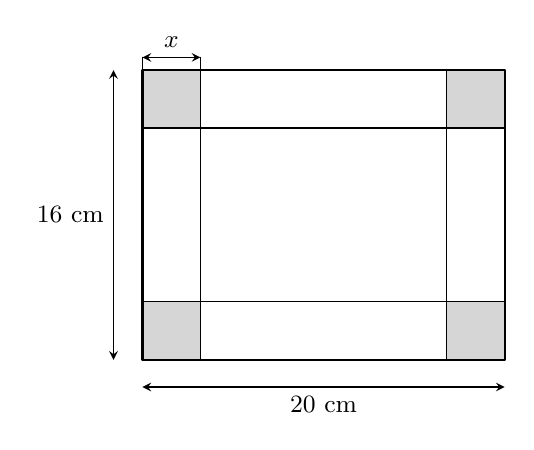
\begin{tikzpicture}[x=0.23cm, y=0.23cm, font=\small, line join=round, line cap=round, >=stealth]
	\fill[gray!32] (0,0) rectangle (3.2,3.2);
	\fill[gray!32] (16.8,0) rectangle (20,3.2);
	\fill[gray!32] (0,12.8) rectangle (3.2,16);
	\fill[gray!32] (16.8,12.8) rectangle (20,16);
	\draw[thick] (0,0) rectangle (20,16);
	\draw (3.2,0)--(3.2,16) (16.8,0)--(16.8,16);
	\draw (0,3.2)--(20,3.2) (0,12.8)--(20,12.8);
	\draw[<->] (0,-1.5)--(20,-1.5) node[midway,below] {$20$ cm};
	\draw[<->] (-1.6,0)--(-1.6,16) node[midway,left] {$16$ cm};
	\draw[<->] (0,16.7)--(3.2,16.7) node[midway,above] {$x$};
	\draw (0,16)--(0,16.7) (3.2,16)--(3.2,16.7);
\end{tikzpicture}
\end{center}
\begin{enumerate}
\item Viết biểu thức diện tích bốn hình vuông bị cắt và diện tích mặt đáy hộp theo $x$.
\item Biết diện tích mặt đáy hộp là $192$ cm$^2$. Tìm $x$.
\end{enumerate}
\loigiai{
\begin{enumerate}
\item Bốn hình vuông bị cắt có tổng diện tích
\[
S_{\text{cắt}}=4x^2\ \text{(cm}^2\text{)}.
\]
Sau khi cắt, mặt đáy có chiều dài $20-2x$ (cm) và chiều rộng $16-2x$ (cm). Diện tích mặt đáy là
\begin{align*}
S_{\text{đáy}}
&=(20-2x)(16-2x)\\
&=4(10-x)(8-x)\\
&=4\bigl(80-18x+x^2\bigr)\\
&=4x^2-72x+320\ \text{(cm}^2\text{)}.
\end{align*}

\item Ta có
\begin{align*}
(20-2x)(16-2x)&=192\\
4(10-x)(8-x)&=192\\
(10-x)(8-x)&=48\\
80-18x+x^2&=48\\
x^2-18x+32&=0\\
(x-16)(x-2)&=0.
\end{align*}
Suy ra $x=16$ hoặc $x=2$.

Vì $0<x<8$ nên $x=16$ bị loại. Với $x=2$, mặt đáy có kích thước $16$ cm và $12$ cm.

\emph{Kiểm tra.} Diện tích mặt đáy là $16\cdot 12=192$ (cm$^2$).

Vậy $x=2$ cm.
\end{enumerate}
}
\end{bt}

%%Bài 5:
\begin{bt}[1,0 điểm]
Một vòi phun nước tưới một vùng đất hình quạt tròn tâm $O$, góc ở tâm $\widehat{AOB}=120^\circ$. Độ dài cung $AB$ là $8\pi$ m (hình vẽ).
\begin{center}
\begin{tikzpicture}[scale=1.15, font=\small, line join=round, line cap=round]
	\coordinate (O) at (0,0);
	\coordinate (A) at (0:3);
	\coordinate (B) at (120:3);
	\fill[blue!8] (O)--(A) arc (0:120:3) -- cycle;
	\draw[thick] (O)--(A) arc (0:120:3) -- cycle;
	\pic[draw, angle radius=0.85cm, angle eccentricity=1.45] {angle = A--O--B};
	\node at (60:1.45) {$120^\circ$};
	\node at (60:3.45) {$8\pi$ m};
	\fill (O) circle (1.1pt) node[below] {$O$};
	\fill (A) circle (1.1pt) node[right] {$A$};
	\fill (B) circle (1.1pt) node[above left] {$B$};
\end{tikzpicture}
\end{center}
\begin{enumerate}
\item Tính bán kính của vùng đất được tưới.
\item Tính diện tích vùng đất được tưới.
\end{enumerate}
\loigiai{
\begin{enumerate}
\item Gọi $R$ (m) là bán kính vùng đất, $R>0$. Độ dài cung $AB$ chắn góc ở tâm $120^\circ$ là
\begin{align*}
\dfrac{\pi R\cdot 120}{180}&=8\pi\\
\dfrac{2R}{3}&=8\\
R&=12.
\end{align*}
Vậy bán kính vùng đất được tưới là $12$ m.

\item Diện tích hình quạt bán kính $12$ m, góc ở tâm $120^\circ$, là
\begin{align*}
S
&=\dfrac{\pi R^2 n}{360}\\
&=\dfrac{\pi\cdot 12^2\cdot 120}{360}\\
&=\dfrac{\pi\cdot 144}{3}\\
&=48\pi\ \text{(m}^2\text{)}.
\end{align*}
Vậy diện tích vùng đất được tưới là $48\pi$ m$^2$.
\end{enumerate}
}
\end{bt}

%%Bài 6:
\begin{bt}[0,5 điểm]
Giải bất phương trình sau: 
\[\dfrac{x+2021}{2022}+\dfrac{x+2022}{2023}<\dfrac{x+2023}{2024}+\dfrac{x+2024}{2025}\]
\loigiai{
$x=1$

Gợi ý: cộng hai vế của phương trình với -2: 
\[\dfrac{x-1}{2022}+\dfrac{x-1}{2023}>\dfrac{x-1}{2024}+\dfrac{x-1}{2025}\]
}
\end{bt}

\Closesolutionfile{ansbook}


	%	%------------------------%
		
		\part{ĐÁP SỐ VÀ LỜI GIẢI}
		\setcounter{section}{0}
	

	    
	    \section{Đề 6}
	        \inputansbox{10}{ans/ans6}
	        \begin{Solbook}{1}
 \par \noindent  \begin {enumerate} \item Điều kiện xác định: $x\ne 2$, $x\ne -2$. \begin {align*} \dfrac {3x+5}{x-2}-\dfrac {3x-1}{x+2}&=\dfrac {26}{x^2-4}\\ (3x+5)(x+2)-(3x-1)(x-2)&=26\\ 18x+8&=26\\ x&=1. \end {align*} Giá trị $x=1$ thỏa mãn điều kiện xác định. Vậy phương trình có nghiệm $x=1$. \par \item Nhân cả hai vế với $12>0$, ta được \begin {align*} 4(2x-3)-3(5x+1)&\ge 2(1-2x)\\ 8x-12-15x-3&\ge 2-4x\\ -3x&\ge 17\\ x&\le -\dfrac {17}{3}. \end {align*} Vậy bất phương trình có nghiệm $x\le -\dfrac {17}{3}$. \par \item Dùng phương pháp thế, ta có \begin {align*} &\begin {cases} 2(x-1)-3(y+2)=-11,\\ \dfrac {x+2y}{3}+\dfrac {x-y}{2}=3 \end {cases}\\[0.7em] \Leftrightarrow \quad &\begin {cases} 2x-3y=-3,\\ 5x+y=18 \end {cases}\\[0.7em] \Leftrightarrow \quad &\begin {cases} 2x-3(18-5x)=-3,\\ y=18-5x \end {cases}\\[0.7em] \Leftrightarrow \quad &\begin {cases} 17x=51,\\ y=18-5x \end {cases}\\[0.7em] \Leftrightarrow \quad &\begin {cases} x=3,\\ y=3. \end {cases} \end {align*} Vậy hệ phương trình có nghiệm $(x;y)=(3;3)$. \end {enumerate}  \hfill \qedEX 
\end{Solbook}
\begin{Solbook}{2}
 \par \noindent  \begin {enumerate} \setlength {\itemsep }{1em} \par \item Ta có \begin {align*} 14+6\sqrt {5} &=9+2\cdot 3\sqrt {5}+5\\ &=\left (3+\sqrt {5}\right )^2,\\ 17-12\sqrt {2} &=9-2\cdot 3\cdot 2\sqrt {2}+8\\ &=\left (3-2\sqrt {2}\right )^2. \end {align*} Vì $3-2\sqrt {2}>0$ nên \begin {align*} \sqrt {14+6\sqrt {5}}-\sqrt {17-12\sqrt {2}} &=\sqrt {\left (3+\sqrt {5}\right )^2} -\sqrt {\left (3-2\sqrt {2}\right )^2}\\ &=3+\sqrt {5}-\left (3-2\sqrt {2}\right )\\ &=\sqrt {5}+2\sqrt {2}. \end {align*} Vậy biểu thức đã cho rút gọn thành $\sqrt {5}+2\sqrt {2}$. \par \item Ta có $\sqrt {45}=3\sqrt {5}$, do đó \begin {align*} \dfrac {\sqrt {45}+\sqrt {5}}{\sqrt {5}-\sqrt {3}} -\dfrac {4\sqrt {3}}{\sqrt {5}+\sqrt {3}}\\ &=\dfrac {4\sqrt {5}}{\sqrt {5}-\sqrt {3}} -\dfrac {4\sqrt {3}}{\sqrt {5}+\sqrt {3}}\\ &=\dfrac {4\sqrt {5}\left (\sqrt {5}+\sqrt {3}\right )}{5-3} -\dfrac {4\sqrt {3}\left (\sqrt {5}-\sqrt {3}\right )}{5-3}\\ &=10+2\sqrt {15}-\left (2\sqrt {15}-6\right )\\ &=16. \end {align*} Vậy biểu thức đã cho rút gọn thành $16$. \end {enumerate}  \hfill \qedEX 
\end{Solbook}
\begin{Solbook}{3}
 \par \noindent  \begin {enumerate} \item Vì hãng A thu $200$ nghìn đồng tiền mở cửa và $4$ nghìn đồng cho mỗi kilômét nên \[ f(x)=4x+200. \] Vì hãng B thu $80$ nghìn đồng tiền mở cửa và $6$ nghìn đồng cho mỗi kilômét nên \[ g(x)=6x+80. \] \par \item Hai hãng có số tiền thuê bằng nhau khi $f(x)=g(x)$. Ta có \begin {align*} 4x+200&=6x+80\\ 200-80&=6x-4x\\ 120&=2x\\ x&=60. \end {align*} Vậy hai hãng thu cùng số tiền khi quãng đường dài $60$ km. \par Xét hiệu \begin {align*} f(x)-g(x) &=(4x+200)-(6x+80)\\ &=120-2x\\ &=2(60-x). \end {align*} Với $x>60$ thì $60-x<0$, nên $f(x)-g(x)<0$, tức là $f(x)<g(x)$. \par Do đó, nếu quãng đường dài hơn $60$ km thì nên chọn hãng A để tiết kiệm chi phí. \end {enumerate}  \hfill \qedEX 
\end{Solbook}
\begin{Solbook}{4}
 \par \noindent  \begin {enumerate} \item Gọi $x$ (nghìn đồng) là giá niêm yết của nồi cơm điện và $y$ (nghìn đồng) là giá niêm yết của bàn là, với $x>0$, $y>0$. \par Tổng giá niêm yết là $750$ nghìn đồng, nên \[ x+y=750. \tag {1} \] Số tiền được giảm là $20\%$ giá nồi cộng với $10\%$ giá bàn là và bằng $120$ nghìn đồng, nên \[ \dfrac {20}{100}x+\dfrac {10}{100}y=120, \] tức là \[ 0{,}2x+0{,}1y=120. \] Nhân hai vế với $10$, ta được \[ 2x+y=1200. \tag {2} \] Lấy $(2)$ trừ $(1)$: \begin {align*} (2x+y)-(x+y)&=1200-750\\ x&=450. \end {align*} Thay $x=450$ vào $(1)$: \[ 450+y=750 \Rightarrow y=300. \] Cặp $(x;y)=(450;300)$ thỏa điều kiện $x>0$, $y>0$. \par Vậy giá niêm yết của nồi cơm điện là $450\,000$ đồng và giá niêm yết của bàn là là $300\,000$ đồng. \par \item Sau khi giảm giá, số tiền thực tế là \begin {align*} \text {nồi cơm điện: }&450\,000\cdot (100\%-20\%)=450\,000\cdot 0{,}8=360\,000 \text { (đồng)},\\ \text {bàn là: }&300\,000\cdot (100\%-10\%)=300\,000\cdot 0{,}9=270\,000 \text { (đồng)}. \end {align*} Vậy phải trả $360\,000$ đồng cho nồi cơm điện và $270\,000$ đồng cho bàn là. \par \emph {Kiểm tra.} Số tiền giảm là $90\,000+30\,000=120\,000$ (đồng), đúng với giả thiết. \end {enumerate}  \hfill \qedEX 
\end{Solbook}
\begin{Solbook}{5}
 \par \noindent  \begin {enumerate} \item Gọi $M$ là vị trí mắt, $A$ là gốc cột đèn, $B$ là đỉnh cột đèn. Kẻ $MH$ vuông góc với $AB$ tại $H$. Khi đó $MH$ song song với mặt đất, $MH=12$ m và $AH=1{,}5$ m. \par Tam giác $MHB$ vuông tại $H$, $\widehat {HMB}=30^\circ $, cạnh đối của góc này là $HB$ và cạnh kề là $MH$. Do đó \[ \tan 30^\circ =\dfrac {HB}{MH} \Rightarrow HB=MH\cdot \tan 30^\circ =12\cdot \dfrac {\sqrt {3}}{3}=4\sqrt {3}\ \text {(m)}. \] Chiều cao cột đèn là \[ AB=AH+HB=1{,}5+4\sqrt {3}\ \text {(m)}. \] Vì $\sqrt {3}\approx 1{,}732$ nên $4\sqrt {3}\approx 6{,}928$ và \[ AB\approx 1{,}5+6{,}928=8{,}428\approx 8{,}4\ \text {(m)}. \] Vậy chiều cao cột đèn khoảng $8{,}4$ m. \par \item Phần cột đèn nằm phía trên tầm mắt vẫn là $HB=4\sqrt {3}$ m. \par Gọi $d$ (m) là khoảng cách từ học sinh đến gốc cột đèn, $d>0$. Tia nhìn tạo với phương nằm ngang góc $45^\circ $ nên \[ \tan 45^\circ =\dfrac {4\sqrt {3}}{d}. \] Vì $\tan 45^\circ =1$ nên $d=4\sqrt {3}$. \par Vậy học sinh phải đứng cách gốc cột đèn $4\sqrt {3}$ m. \end {enumerate}  \hfill \qedEX 
\end{Solbook}
\begin{Solbook}{6}
 \par \noindent  \immini { \begin {enumerate} \item $A,P,O,M$ cùng nằm trên đường tròn đường kính $OP$ \par Ta có $OP\perp AM, BM\perp AM$ suy ra $OP\parallel BM$. \item $\triangle AOP = \triangle OBN \Rightarrow OP = BN$ \par Ta lại có $BN \parallel OP$ nên $OBNP$ là hình bình hành. \par \item Chứng minh $I$ là trực tâm $\triangle POJ$ suy ra $IJ \perp OP$ (1) \par Chứng minh $K$ là trung điểm $OP$. \par Lại có: $\widehat {APO} = \widehat {OPI} = \widehat {IOP}$ \par Suy ra $\triangle IPO$ cân tại $I$ suy ra $IK \perp OP$ (2) \par Từ (1) và (2) suy ra $I, J, K$ thẳng hàng. \end {enumerate} } { \begin {tikzpicture}[scale=1, font=\footnotesize , line join =round, line cap=round, >=stealth] \def \r {1.8} \path (0,0) coordinate (O) (180:\r ) coordinate (A) (0:\r ) coordinate (B) (-\r ,2.5*\r ) coordinate (x)node[left]{$x$} ($(A)!4/5!(x)$) coordinate (P) ($(O)!(A)!(P)$) coordinate (H) ($(A)!2!(H)$) coordinate (M) ($(O)!1cm!-90:(A)$) coordinate (n') (intersection of B--M and O--n') coordinate (N) (intersection of A--N and O--P) coordinate (K) (intersection of O--N and M--P) coordinate (I) (intersection of O--M and N--P) coordinate (J) ; \draw (O) circle (\r ) (x)--(A)--(B)--(N)--(A)--(M)--(P)--(O)--(N) (P)--(J)--(O) ; \draw [dashed] (K)--(J); \foreach \x /\g in{O/-90,A/180,B/0,P/180,K/160,M/0,N/90,I/120,J/40} \draw [fill=white] (\x ) circle (1.5pt) +(\g :.3) node{$\x $}; \end {tikzpicture} }  \hfill \qedEX 
\end{Solbook}

	    
	    \section{Đề 7}
	        \inputansbox{10}{ans/ans7}
	        \begin{Solbook}{1}
 \par \noindent  \begin {enumerate} \item Ta có \begin {align*} (3x-2)^2-(x+4)^2&=0\\ \big [(3x-2)-(x+4)\big ]\big [(3x-2)+(x+4)\big ]&=0\\ (2x-6)(4x+2)&=0. \end {align*} Do đó $x=3$ hoặc $x=-\dfrac {1}{2}$. \par \item Nhân cả hai vế với $12>0$, ta được \begin {align*} 3(3x-2)-4(x+5)&<2(5x+1)\\ 5x-26&<10x+2\\ -28&<5x\\ x&>-\dfrac {28}{5}. \end {align*} Vậy bất phương trình có nghiệm $x>-\dfrac {28}{5}$. \par \item Dùng phương pháp cộng đại số, ta có \begin {align*} &\begin {cases} \dfrac {2x-y}{3}+\dfrac {x+2y}{2}=\dfrac {5}{3},\\ 3(x-1)-2(y+2)=1 \end {cases}\\[0.7em] \Leftrightarrow \quad &\begin {cases} 7x+4y=10,\\ 3x-2y=8 \end {cases}\\[0.7em] \Leftrightarrow \quad &\begin {cases} 7x+4y=10,\\ 6x-4y=16 \end {cases}\\[0.7em] \Leftrightarrow \quad &\begin {cases} 13x=26,\\ 3x-2y=8 \end {cases}\\[0.7em] \Leftrightarrow \quad &\begin {cases} x=2,\\ y=-1. \end {cases} \end {align*} Vậy hệ phương trình có nghiệm $(x;y)=(2;-1)$. \end {enumerate}  \hfill \qedEX 
\end{Solbook}
\begin{Solbook}{2}
 \par \noindent  \begin {enumerate} \setlength {\itemsep }{1em} \par \item Ta có \begin {align*} 23+8\sqrt {7} &=16+2\cdot 4\sqrt {7}+7\\ &=\left (4+\sqrt {7}\right )^2,\\ 23-8\sqrt {7} &=16-2\cdot 4\sqrt {7}+7\\ &=\left (4-\sqrt {7}\right )^2,\\ 14-4\sqrt {10} &=10-2\cdot \sqrt {10}\cdot 2+4\\ &=\left (\sqrt {10}-2\right )^2. \end {align*} Vì $4-\sqrt {7}>0$ và $\sqrt {10}-2>0$ nên \begin {align*} \sqrt {23+8\sqrt {7}}+\sqrt {23-8\sqrt {7}} -\sqrt {14-4\sqrt {10}}\\ &=4+\sqrt {7}+4-\sqrt {7}-\left (\sqrt {10}-2\right )\\ &=10-\sqrt {10}. \end {align*} Vậy biểu thức đã cho rút gọn thành $10-\sqrt {10}$. \par \item Ta có $\sqrt {80}=4\sqrt {5}$, do đó \begin {align*} \dfrac {\sqrt {80}-\sqrt {5}}{\sqrt {5}-\sqrt {3}} +\dfrac {3\sqrt {3}}{\sqrt {5}+\sqrt {3}}\\ &=\dfrac {3\sqrt {5}}{\sqrt {5}-\sqrt {3}} +\dfrac {3\sqrt {3}}{\sqrt {5}+\sqrt {3}}\\ &=\dfrac {3\sqrt {5}\left (\sqrt {5}+\sqrt {3}\right )}{5-3} +\dfrac {3\sqrt {3}\left (\sqrt {5}-\sqrt {3}\right )}{5-3}\\ &=\dfrac {15+3\sqrt {15}+3\sqrt {15}-9}{2}\\ &=3+3\sqrt {15}. \end {align*} Vậy biểu thức đã cho rút gọn thành $3+3\sqrt {15}$. \end {enumerate}  \hfill \qedEX 
\end{Solbook}
\begin{Solbook}{3}
 \par \noindent  Gọi $x$ (km/h) và $y$ (h) lần lượt là vận tốc dự định và thời gian dự định. \par Quãng đường AB là 600 km, xe xuất phát lúc 7 giờ tối hôm trước.  \hfill \qedEX 
\end{Solbook}
\begin{Solbook}{4}
 \par \noindent  \immini {\begin {enumerate} \item $A,M,C,K$ thuộc đường tròn tâm $I$ bán kính $IM$. \item $\triangle MHB=\triangle NHB$, suy ra $\widehat {MBH}=\widehat {NBH}$. \item $\triangle KMH=\triangle KNH$, suy ra $KM=NK$ \par $\widehat {KMO}=180^\circ -\widehat {KMC}-\widehat {OMB}=180-\widehat {KCM}-\widehat {OBM}=\widehat {CKB}=90^\circ $ \end {enumerate}} {\begin {tikzpicture}[line cap=round,line join=round,font=\footnotesize ] \def \r {2} \path (-\r ,0) coordinate (A) (\r ,0) coordinate (B) (0,0) coordinate (O) ($(O)!1!-50:(A)$) coordinate (M) ($(A)!(M)!(B)$) coordinate (H) ($(M)!2!(H)$) coordinate (N) ($(B)!2!(M)$) coordinate (Bt) ($(N)!2.5!(A)$) coordinate (Nt) (intersection of N--Nt and B--Bt) coordinate (C) ($(A)!(C)!(B)$) coordinate (K) ($(C)!2!(K)$) coordinate (Ct) ($(B)!1.5!(N)$) coordinate (Nt) (intersection of C--Ct and B--Nt) coordinate (D) ($(C)!0.5!(A)$) coordinate (I) ; \draw (O) circle (\r ) (M)--(N) (K)--(A)--(B)--(C)--(D)--(B) (C)--(N) (M)--(A)--(B)--cycle (M)--(I)--(K) (M)--(O)--(N)--(K)--(M) ; \foreach \x /\g in{A/-135,B/-45,O/-90,M/90,H/-45,N/-90,C/90,K/180,D/-90,I/70} \draw [fill=white] (\x ) circle (1.5pt) +(\g :.35) node{$\x $}; \end {tikzpicture}}  \hfill \qedEX 
\end{Solbook}
\begin{Solbook}{5}
 \par \noindent  $x$ (triệu đồng) là số tiền ban đầu người đó gửi vào ngân hàng \par $0,5\%\left (1+0,5\%\right )\ge 0,5$ \par Người đó cần gửi số tiền ban đầu ít nhất là 100 triệu đồng.  \hfill \qedEX 
\end{Solbook}

	    
	    \section{Đề 8}
	        \inputansbox{10}{ans/ans8}
	        \begin{Solbook}{1}
 \par \noindent  \begin {enumerate} \item Điều kiện xác định: $x\ne 1$, $x\ne -1$. \begin {align*} \dfrac {x+2}{x-1}+\dfrac {x-3}{x+1}&=\dfrac {4x+2}{x^2-1}\\ (x+2)(x+1)+(x-3)(x-1)&=4x+2\\ 2x^2-5x+3&=0\\ (2x-3)(x-1)&=0. \end {align*} Suy ra $x=\dfrac {3}{2}$ hoặc $x=1$. \\ Vì $x=1$ không thỏa mãn điều kiện xác định nên phương trình có nghiệm $x=\dfrac {3}{2}$. \par \item Nhân cả hai vế với $6>0$, ta được \begin {align*} 2(2x-3)-3(x+4)&\le 5(x-2)\\ x-18&\le 5x-10\\ -8&\le 4x\\ x&\ge -2. \end {align*} Vậy bất phương trình có nghiệm $x\ge -2$. \par \item Dùng phương pháp thế, ta có \begin {align*} &\begin {cases} (x+2)(y-1)=xy-6,\\ (x-1)(y+3)=xy+4 \end {cases}\\[0.7em] \Leftrightarrow \quad &\begin {cases} x-2y=4,\\ 3x-y=7 \end {cases}\\[0.7em] \Leftrightarrow \quad &\begin {cases} x=4+2y,\\ 3x-y=7 \end {cases}\\[0.7em] \Leftrightarrow \quad &\begin {cases} x=4+2y,\\ 3(4+2y)-y=7 \end {cases}\\[0.7em] \Leftrightarrow \quad &\begin {cases} x=4+2y,\\ 5y=-5 \end {cases}\\[0.7em] \Leftrightarrow \quad &\begin {cases} x=2,\\ y=-1. \end {cases} \end {align*} Vậy hệ phương trình có nghiệm $(x;y)=(2;-1)$. \end {enumerate}  \hfill \qedEX 
\end{Solbook}
\begin{Solbook}{2}
 \par \noindent  \begin {enumerate} \setlength {\itemsep }{1em} \par \item Ta có \begin {align*} x+6\sqrt {x}+9&=\left (\sqrt {x}+3\right )^2,\\ x-4\sqrt {x}+4&=\left (\sqrt {x}-2\right )^2,\\ x-10\sqrt {x}+25&=\left (\sqrt {x}-5\right )^2. \end {align*} Vì $4\le x\le 25$ nên $2\le \sqrt {x}\le 5$. Do đó \begin {align*} A &=\left |\sqrt {x}+3\right | +\left |\sqrt {x}-2\right | -\left |\sqrt {x}-5\right |\\ &=\sqrt {x}+3+\sqrt {x}-2-\left (5-\sqrt {x}\right )\\ &=3\sqrt {x}-4. \end {align*} Vậy $A=3\sqrt {x}-4$. \par \item Với $x\ge 0$ và $x\ne 4$, ta có \begin {align*} B &=\left (\dfrac {\sqrt {x}+2}{\sqrt {x}-2} -\dfrac {\sqrt {x}-2}{\sqrt {x}+2}\right ) \cdot \dfrac {x-4}{8}\\ &=\dfrac {\left (\sqrt {x}+2\right )^2 -\left (\sqrt {x}-2\right )^2}{x-4} \cdot \dfrac {x-4}{8}\\ &=\dfrac {8\sqrt {x}}{x-4}\cdot \dfrac {x-4}{8}\\ &=\sqrt {x}. \end {align*} Vậy $B=\sqrt {x}$. \end {enumerate}  \hfill \qedEX 
\end{Solbook}
\begin{Solbook}{3}
 \par \noindent  Gọi $x$ (nghìn đồng) là giá một vé người lớn buổi sáng và $y$ (nghìn đồng) là giá một vé trẻ em buổi sáng, với $x>0$, $y>0$. \par Buổi sáng cho ta \[ 3x+2y=400. \tag {1} \] Buổi chiều, vé người lớn có giá $\dfrac {3}{4}x$ và vé trẻ em có giá $\dfrac {9}{10}y$, nên \[ 4\cdot \dfrac {3}{4}x+2\cdot \dfrac {9}{10}y=390, \] tức là \[ 3x+\dfrac {9}{5}y=390. \] Nhân hai vế với $5$: \[ 15x+9y=1950. \] Chia hai vế cho $3$: \[ 5x+3y=650. \tag {2} \] Nhân $(2)$ với $2$ và nhân $(1)$ với $3$: \begin {align*} 10x+6y&=1300, \tag {3}\\ 9x+6y&=1200. \tag {4} \end {align*} Lấy $(3)$ trừ $(4)$: \[ x=100. \] Thay vào $(1)$: \[ 3\cdot 100+2y=400 \Rightarrow 2y=100 \Rightarrow y=50. \] Cặp $(x;y)=(100;50)$ thỏa $x>0$, $y>0$. \par \emph {Kiểm tra.} Buổi chiều, vé người lớn giá $75$ nghìn đồng và vé trẻ em giá $45$ nghìn đồng. \[ 4\cdot 75+2\cdot 45=300+90=390, \] đúng với giả thiết. \par Vậy buổi sáng, một vé người lớn giá $100\,000$ đồng và một vé trẻ em giá $50\,000$ đồng.  \hfill \qedEX 
\end{Solbook}
\begin{Solbook}{4}
 \par \noindent  \begin {enumerate} \item Diện tích hình chữ nhật là \[ S_{\text {cn}}=(x+5)(x+1)=x^2+6x+5\ \text {(cm}^2\text {)}. \] Diện tích hình tròn bán kính $2$ cm là \[ S_{\text {tròn}}=\pi \cdot 2^2=4\pi \ \text {(cm}^2\text {)}. \] Diện tích phần tô đậm là \[ S=S_{\text {cn}}-S_{\text {tròn}}=x^2+6x+5-4\pi \ \text {(cm}^2\text {)}. \] \par \item Ta có \begin {align*} x^2+6x+5-4\pi &=32-4\pi \\ x^2+6x+5&=32\\ x^2+6x-27&=0\\ (x+9)(x-3)&=0. \end {align*} Suy ra $x=-9$ hoặc $x=3$. \par Vì $x>0$ nên $x=-9$ bị loại. Với $x=3$, hình chữ nhật có chiều dài $8$ cm và chiều rộng $4$ cm. Đường kính hình tròn bằng $4$ cm nên hình tròn tiếp xúc hai cạnh chiều rộng và nằm trọn trong hình chữ nhật. \par Vậy $x=3$ cm. \end {enumerate}  \hfill \qedEX 
\end{Solbook}
\begin{Solbook}{5}
 \par \noindent  \begin {enumerate} \item Gọi $R$ (m) là bán kính mép ngoài, $R>5$. Diện tích hình vành khuyên là \begin {align*} \pi R^2-\pi \cdot 5^2&=75\pi \\ R^2-25&=75\\ R^2&=100. \end {align*} Vì $R>0$ nên $R=10$. \par Vậy bán kính mép ngoài là $10$ m. \par \item Cung nhỏ $AB$ thuộc đường tròn bán kính $10$ m và chắn góc ở tâm $60^\circ $, nên \[ \ell _{\overset {\frown }{AB}} =\dfrac {\pi Rn}{180} =\dfrac {\pi \cdot 10\cdot 60}{180} =\dfrac {10\pi }{3}\ \text {(m)}. \] Phần đường chạy trong góc $\widehat {AOB}$ là hình quạt vành khuyên, bằng hiệu hai hình quạt cùng góc $60^\circ $: \begin {align*} S &=\dfrac {60}{360}\pi \cdot 10^2-\dfrac {60}{360}\pi \cdot 5^2\\ &=\dfrac {1}{6}\pi (100-25)\\ &=\dfrac {75\pi }{6} =\dfrac {25\pi }{2}\ \text {(m}^2\text {)}. \end {align*} Vậy cung nhỏ $AB$ dài $\dfrac {10\pi }{3}$ m và phần đường chạy trong góc $\widehat {AOB}$ có diện tích $\dfrac {25\pi }{2}$ m$^2$. \end {enumerate}  \hfill \qedEX 
\end{Solbook}
\begin{Solbook}{6}
 \par \noindent  \begin {center} \begin {tikzpicture}[scale=1.1, font=\footnotesize , line join=round, line cap=round] \coordinate (O) at (0,0); \coordinate (A) at (0,4); \coordinate (B) at (-1.732,1); \coordinate (C) at (1.732,1); \coordinate (H) at (0,1); \coordinate (M) at (-0.866,2.5); \coordinate (N) at (0.866,2.5); \coordinate (D) at (-0.684,1.879); \coordinate (I) at (1.020,2.5); \coordinate (T) at (0.560,1.372); \par \draw [thick] (O) circle (2); \par \draw [thick] (A)--(B) (A)--(C); \draw [thick] (B)--(C); \draw [thick] (O)--(A); \draw [thick] (M)--(I); \draw [thick] (D)--(I); \par \draw [dashed] (O)--(B) (O)--(C) (O)--(D) (O)--(I) (D)--(T); \par \draw ($(T)+(0.08,0.03)$)--++(-0.09,0.12)--++(-0.12,-0.09); \draw ($(H)+(-0.08,0)$)--++(0,0.08)--++(0.08,0); \par \fill (A) circle (1.2pt) node[above] {$A$}; \fill (O) circle (1.2pt) node[left] {$O$}; \fill (B) circle (1.2pt) node[left] {$B$}; \fill (C) circle (1.2pt) node[right] {$C$}; \fill (H) circle (1.2pt) node[right] {$H$}; \fill (M) circle (1.2pt) node[left] {$M$}; \fill (N) circle (1.2pt) node[above] {$N$}; \fill (D) circle (1.2pt) node[above left] {$D$}; \fill (I) circle (1.2pt) node[right] {$I$}; \fill (T) circle (1.2pt) node[right] {$T$}; \end {tikzpicture} \end {center} \par \begin {enumerate} \item Vì $AB$, $AC$ là hai tiếp tuyến kẻ từ $A$ đến đường tròn $(O)$ nên \[ AB=AC. \] Mặt khác, \[ OB=OC \] (vì cùng bằng bán kính của đường tròn $(O)$). \par Vậy $A$ và $O$ đều cách đều hai điểm $B$, $C$, suy ra đường thẳng $AO$ là đường trung trực của đoạn thẳng $BC$. \par Do đó \[ OA\perp BC. \] \par \item Từ câu a), ta có $OA\perp BC$. Lại do $AO$ là đường trung trực của $BC$ nên \[ HB=HC=\dfrac {BC}{2}. \tag {1} \] \par Xét hai tam giác vuông $\triangle AHB$ và $\triangle AOB$, ta có: \begin {itemize} \item $\widehat {AHB}=90^\circ $; \item $\widehat {ABO}=90^\circ $ (bán kính vuông góc với tiếp tuyến); \item $\widehat {BAH}=\widehat {BAO}$. \end {itemize} Suy ra \[ \triangle AHB \sim \triangle AOB. \] \par Do đó \[ \dfrac {AH}{AB}=\dfrac {AB}{AO} \Rightarrow AH\cdot AO=AB^2. \tag {2} \] \par Mà trong tam giác vuông $AOB$, ta có \[ AB^2=AO^2-OB^2=AO^2-R^2. \] Thay vào (2), được \[ AH\cdot AO=AO^2-R^2. \] Suy ra \[ AO(AO-AH)=R^2. \] Vì $O,H,A$ thẳng hàng và $H$ nằm giữa $O,A$ nên \[ AO-AH=OH. \] Do đó \[ OA\cdot OH=R^2. \tag {3} \] \par Xét tam giác vuông $OHB$, ta có \[ HB^2=OB^2-OH^2=R^2-OH^2. \] Theo (3), $R^2=OA\cdot OH$, nên \[ HB^2=OA\cdot OH-OH^2=OH(OA-OH). \] Mà $OA-OH=HA$, suy ra \[ HB^2=OH\cdot HA. \] Nhân hai vế với $4$, ta được \[ 4HB^2=4OH\cdot HA. \] Theo (1), \[ BC=2HB \Rightarrow BC^2=4HB^2. \] Vậy \[ 4OH\cdot HA=BC^2. \] \par \item Gọi $K=OA\cap MN$. \par Vì $M$, $N$ lần lượt là trung điểm của $AB$, $AC$ nên trong tam giác $ABC$ ta có \[ MN\parallel BC. \] Suy ra \[ OA\perp MN \tag {4} \] (do $OA\perp BC$ theo câu a)). \par Lại vì $MN\parallel BC$, nên $\triangle AMN \sim \triangle ABC$ với tỉ số đồng dạng \[ \dfrac {AM}{AB}=\dfrac 12. \] Do đó \[ \dfrac {AK}{AH}=\dfrac 12 \Rightarrow AK=\dfrac {AH}{2}. \] Suy ra $K$ là trung điểm của $AH$, nên \[ AK=KH=\dfrac {AH}{2}. \tag {5} \] \par \medskip \textbf {Chứng minh $OH\cdot OA=OT\cdot OI$.} \par Vì $ID$ là tiếp tuyến của $(O)$ tại $D$ nên \[ OD\perp ID. \] Suy ra tam giác $ODI$ vuông tại $D$. \par Lại có $T$ là hình chiếu của $D$ trên $OI$, nên \[ DT\perp OI. \] Vậy $DT$ là đường cao ứng với cạnh huyền $OI$ của tam giác vuông $ODI$. \par Theo hệ thức lượng trong tam giác vuông, ta có \[ OD^2=OT\cdot OI. \] Mà $OD=R$, nên \[ R^2=OT\cdot OI. \tag {6} \] \par Mặt khác, theo (3), \[ OH\cdot OA=R^2. \tag {7} \] \par Từ (6) và (7), suy ra \[ OH\cdot OA=OT\cdot OI. \] \par \medskip \textbf {Chứng minh $IA=ID$.} \par Do $I\in MN$ và $K\in MN$, từ (4) suy ra hai tam giác $AKI$ và $OKI$ đều vuông tại $K$. \par Áp dụng định lý Py-ta-go, ta có \[ IA^2=IK^2+AK^2, \tag {8} \] \[ OI^2=IK^2+OK^2. \tag {9} \] \par Lấy (9) trừ (8), được \[ OI^2-IA^2=OK^2-AK^2=(OK-AK)(OK+AK). \tag {10} \] \par Từ (5), vì $K$ là trung điểm của $AH$ và các điểm $O,H,K,A$ thẳng hàng theo thứ tự đó, nên \[ OK-AK=OH, \qquad OK+AK=OA. \] Thay vào (10), ta được \[ OI^2-IA^2=OH\cdot OA=R^2. \tag {11} \] \par Mặt khác, trong tam giác vuông $ODI$, ta có \[ ID^2=OI^2-OD^2=OI^2-R^2. \tag {12} \] \par Từ (11), suy ra \[ IA^2=OI^2-R^2. \] Kết hợp với (12), ta được \[ IA^2=ID^2. \] Suy ra \[ IA=ID. \] \par Vậy ta đã chứng minh được \[ OH\cdot OA=OT\cdot OI \quad \text {và} \quad IA=ID. \] \end {enumerate}  \hfill \qedEX 
\end{Solbook}

	
	    \section{Đề 9}
	        \inputansbox{10}{ans/ans9}
	        \begin{Solbook}{1}
 \par \noindent  \begin {enumerate} \item Điều kiện xác định: $x\ne 1$, $x\ne -2$. \begin {align*} \dfrac {3x+4}{x-1}-\dfrac {x-2}{x+2}&=\dfrac {19x+14}{x^2+x-2}\\ (3x+4)(x+2)-(x-2)(x-1)&=19x+14\\ 2x^2-6x-8&=0\\ (x-4)(x+1)&=0. \end {align*} Suy ra $x=4$ hoặc $x=-1$; cả hai giá trị đều thỏa mãn điều kiện xác định. Vậy $S=\{-1;4\}$. \par \item Nhân cả hai vế với $4>0$, ta được \begin {align*} -8(3x-5)+2(5x+1)&>3-x\\ -14x+42&>3-x\\ 39&>13x\\ x&<3. \end {align*} Vậy bất phương trình có nghiệm $x<3$. \par \item Dùng phương pháp thế, ta có \begin {align*} &\begin {cases} \dfrac {x+2y}{3}-\dfrac {2x-y}{4}=2,\\ 3(x-y)+2(2x+y)=-9 \end {cases}\\[0.7em] \Leftrightarrow \quad &\begin {cases} -2x+11y=24,\\ 7x-y=-9 \end {cases}\\[0.7em] \Leftrightarrow \quad &\begin {cases} -2x+11y=24,\\ y=7x+9 \end {cases}\\[0.7em] \Leftrightarrow \quad &\begin {cases} -2x+11(7x+9)=24,\\ y=7x+9 \end {cases}\\[0.7em] \Leftrightarrow \quad &\begin {cases} 75x=-75,\\ y=7x+9 \end {cases}\\[0.7em] \Leftrightarrow \quad &\begin {cases} x=-1,\\ y=2. \end {cases} \end {align*} Vậy hệ phương trình có nghiệm $(x;y)=(-1;2)$. \end {enumerate}  \hfill \qedEX 
\end{Solbook}
\begin{Solbook}{2}
 \par \noindent  \begin {enumerate} \setlength {\itemsep }{1em} \par \item Ta có \begin {align*} x+3+4\sqrt {x-1}&=\left (\sqrt {x-1}+2\right )^2,\\ x+3-4\sqrt {x-1}&=\left (\sqrt {x-1}-2\right )^2,\\ 4x-4&=\left (2\sqrt {x-1}\right )^2. \end {align*} Vì $1\le x\le 5$ nên $0\le \sqrt {x-1}\le 2$. Do đó \begin {align*} A &=\left |\sqrt {x-1}+2\right | +\left |\sqrt {x-1}-2\right | -\left |2\sqrt {x-1}\right |\\ &=\sqrt {x-1}+2+2-\sqrt {x-1}-2\sqrt {x-1}\\ &=4-2\sqrt {x-1}. \end {align*} Vậy $A=4-2\sqrt {x-1}$. \par \item Với $x\ge 0$ và $x\ne 4$, ta có \begin {align*} B &=\dfrac {(\sqrt {x}-2)(\sqrt {x}+2)}{\sqrt {x}-2} -\dfrac {(\sqrt {x}-1)(\sqrt {x}+1)}{\sqrt {x}+1} +\dfrac {2}{\sqrt {x}-2}-\dfrac {2}{\sqrt {x}+2}\\ &=\sqrt {x}+2-\left (\sqrt {x}-1\right ) +\dfrac {2(\sqrt {x}+2)-2(\sqrt {x}-2)}{x-4}\\ &=3+\dfrac {8}{x-4}\\ &=\dfrac {3(x-4)+8}{x-4}\\ &=\dfrac {3x-4}{x-4}. \end {align*} Vậy $B=\dfrac {3x-4}{x-4}$. \end {enumerate}  \hfill \qedEX 
\end{Solbook}
\begin{Solbook}{3}
 \par \noindent  Gọi $x$ là số học sinh nam và $y$ là số học sinh nữ của lớp, với $x,y$ nguyên dương và $x+y=36$. \par Tổng chiều cao của cả lớp là $160\cdot 36=5760$ (cm). Tổng chiều cao của các bạn nam là $168x$ (cm) và của các bạn nữ là $156y$ (cm), nên \[ 168x+156y=5760. \tag {1} \] Vì $y=36-x$, thay vào $(1)$: \begin {align*} 168x+156(36-x)&=5760\\ 168x+5616-156x&=5760\\ 12x&=144\\ x&=12. \end {align*} Suy ra $y=36-12=24$. \par \emph {Kiểm tra.} Tổng chiều cao là \[ 168\cdot 12+156\cdot 24=2016+3744=5760\ \text {(cm)}, \] trung bình $5760:36=160$ (cm), đúng với giả thiết. \par Vậy lớp có $12$ học sinh nam và $24$ học sinh nữ.  \hfill \qedEX 
\end{Solbook}
\begin{Solbook}{4}
 \par \noindent  \begin {enumerate} \item Diện tích hình chữ nhật là \[ S_{\text {cn}}=x(x+2)=x^2+2x\ \text {(cm}^2\text {)}. \] Nửa hình tròn có đường kính $x$ cm nên bán kính $\dfrac {x}{2}$ cm. Diện tích nửa hình tròn là \[ S_{\text {nửa}}=\dfrac {1}{2}\pi \left (\dfrac {x}{2}\right )^2=\dfrac {\pi x^2}{8}\ \text {(cm}^2\text {)}. \] Diện tích toàn biển báo là \[ S=S_{\text {cn}}+S_{\text {nửa}}=x^2+2x+\dfrac {\pi x^2}{8}\ \text {(cm}^2\text {)}. \] \par \item Ta có \[ x^2+2x+\dfrac {\pi x^2}{8}=48+\dfrac {9\pi }{2}, \] nên \[ \left (x^2+2x-48\right )+\pi \left (\dfrac {x^2}{8}-\dfrac {9}{2}\right )=0. \] Phần không chứa $\pi $ và hệ số của $\pi $ đều bằng $0$: \begin {align*} \dfrac {x^2}{8}&=\dfrac {9}{2}\\ x^2&=36. \end {align*} Vì $x>0$ nên $x=6$. \par \emph {Kiểm tra.} $x^2+2x=36+12=48$, đúng với phần không chứa $\pi $. \par Vậy $x=6$ cm. \end {enumerate}  \hfill \qedEX 
\end{Solbook}
\begin{Solbook}{5}
 \par \noindent  \begin {enumerate} \item Gọi $M$ là vị trí mắt, $C$ là chân cột ăng-ten, $B$ là đỉnh cột và $A$ là chân tường. Kẻ $MH$ vuông góc với $AB$ tại $H$. Khi đó $MH$ song song với mặt đất, $AH=1{,}5$ m và $BC=6$ m. \par Đặt $MH=d$ (m), $d>0$. \par Tam giác $MHC$ vuông tại $H$, $\widehat {HMC}=30^\circ $, nên \[ \tan 30^\circ =\dfrac {HC}{d} \Rightarrow HC=d\cdot \dfrac {\sqrt {3}}{3}. \] Tam giác $MHB$ vuông tại $H$, $\widehat {HMB}=45^\circ $, nên \[ \tan 45^\circ =\dfrac {HB}{d} \Rightarrow HB=d. \] Vì $B$, $C$, $H$ thẳng hàng và $C$ nằm giữa $H$ và $B$ nên $HB=HC+CB$: \begin {align*} d&=d\cdot \dfrac {\sqrt {3}}{3}+6\\ d\left (1-\dfrac {\sqrt {3}}{3}\right )&=6\\ d\cdot \dfrac {3-\sqrt {3}}{3}&=6\\ d(3-\sqrt {3})&=18\\ d&=\dfrac {18}{3-\sqrt {3}}. \end {align*} Nhân liên hợp với $3+\sqrt {3}$: \[ d=\dfrac {18(3+\sqrt {3})}{(3-\sqrt {3})(3+\sqrt {3})} =\dfrac {18(3+\sqrt {3})}{6} =3(3+\sqrt {3}) =9+3\sqrt {3}. \] Vậy Minh đứng cách mặt tường tòa nhà $9+3\sqrt {3}$ m. \par \item Chiều cao nóc nhà là \begin {align*} AC &=AH+HC\\ &=1{,}5+d\cdot \dfrac {\sqrt {3}}{3}\\ &=1{,}5+(9+3\sqrt {3})\cdot \dfrac {\sqrt {3}}{3}\\ &=1{,}5+\dfrac {9\sqrt {3}+9}{3}\\ &=1{,}5+3\sqrt {3}+3\\ &=4{,}5+3\sqrt {3}\ \text {(m)}. \end {align*} Vậy nóc nhà cao $4{,}5+3\sqrt {3}$ m so với mặt đất. \end {enumerate}  \hfill \qedEX 
\end{Solbook}


	    \section{Đề 10}
	        \inputansbox{10}{ans/ans10}
	        \begin{Solbook}{1}
 \par \noindent  \begin {enumerate} \item Ta có \begin {align*} &(2x-1)^2=9(x-2)^2\\ &(2x-1)^2-\big [3(x-2)\big ]^2=0\\ &\big [(2x-1)-3(x-2)\big ]\big [(2x-1)+3(x-2)\big ]=0\\ &(5-x)(5x-7)=0. \end {align*} Do đó $x=5$ hoặc $x=\dfrac {7}{5}$. \par \item Thu gọn vế phải rồi nhân cả hai vế với $12>0$: \begin {align*} 3-\dfrac {2x-5}{4}&\le \dfrac {x+5}{6}\\ 3(17-2x)&\le 2(x+5)\\ 51-6x&\le 2x+10\\ 41&\le 8x\\ x&\ge \dfrac {41}{8}. \end {align*} Vậy bất phương trình có nghiệm $x\ge \dfrac {41}{8}$. \par \item Dùng phương pháp cộng đại số, ta có \begin {align*} &\begin {cases} \dfrac {3x-y}{4}+\dfrac {x+2y}{3}=\dfrac {1}{6},\\ 2(x+1)-3(y-2)=-3 \end {cases}\\[0.7em] \Leftrightarrow \quad &\begin {cases} 13x+5y=2,\\ 2x-3y=-11 \end {cases}\\[0.7em] \Leftrightarrow \quad &\begin {cases} 39x+15y=6,\\ 10x-15y=-55 \end {cases}\\[0.7em] \Leftrightarrow \quad &\begin {cases} 49x=-49,\\ 2x-3y=-11 \end {cases}\\[0.7em] \Leftrightarrow \quad &\begin {cases} x=-1,\\ y=3. \end {cases} \end {align*} Vậy hệ phương trình có nghiệm $(x;y)=(-1;3)$. \end {enumerate}  \hfill \qedEX 
\end{Solbook}
\begin{Solbook}{2}
 \par \noindent  \noindent a) $A=4$ \par \par \noindent b) $B=\dfrac {5-\sqrt {x}}{\sqrt {x}+5}$  \hfill \qedEX 
\end{Solbook}
\begin{Solbook}{3}
 \par \noindent  Một cái bánh mỳ có giá 20\,000 đồng, một cái bánh bao có giá 25\,000 đồng.  \hfill \qedEX 
\end{Solbook}
\begin{Solbook}{4}
 \par \noindent Khoảng $35{,}7$ km. \hfill \qedEX 
\end{Solbook}
\begin{Solbook}{5}
 \par \noindent \immini {\begin {enumerate} \item $MN$ là đường trung trực của $SO$ \item $\triangle SNF \backsim \triangle SEN$ suy ra $SN^2=SF\cdot SE$ \par $\triangle SNH \backsim \triangle SON$ suy ra $SN^2=SH\cdot SO$ \item $\triangle SHI \backsim \triangle SKO$ suy ra $SK\cdot SI=SH\cdot SO$ \par Chứng minh $SF+SE=2SK$ \par Suy ra $SI(SF+SE)=2SI\cdot SK=2SE\cdot SF$ \end {enumerate}} {\begin {tikzpicture}[scale=1, font=\footnotesize ] \coordinate (O) at (0,0); \def \R {2} \draw (O) circle(\R ); \coordinate (S) at (-5,0); \path [name path=circleO] (O) circle(\R ); \path [name path=circleS] (-2.5,0) circle(2.5); \path [name intersections={of=circleS and circleO, by={M,N}}]; \coordinate (E) at ($-1*(N)$); \path [name path=os] (O)--(S); \path [name path=mn] (M)--(N); \path [name intersections={of=os and mn, by=H}]; \path [name path=se] (S)--(E); \path [name intersections={of=circleO and se, by={F1,F2}}]; \coordinate (F) at (F2); \path [name intersections={of=se and mn, by=I}]; \draw (S)--(M)--(O)--cycle; \draw (M)--(N)--(E)--(S); \draw (S)--(O); \coordinate (K) at ($(F)!0.5!(E)$); \draw (O)--(K); \foreach \p /\pos in {S/left,M/above,N/below,O/below right,F/below,E/above,K/above,I/below left,H/below left} {\draw [fill=white] (\p ) circle(1.5pt) node[\pos ] {$\p $}; } \end {tikzpicture}}  \hfill \qedEX 
\end{Solbook}
\begin{Solbook}{6}
 \par \noindent  $x=1$ \par Gợi ý: cộng hai vế của phương trình với -2: \[\dfrac {x-1}{2022}+\dfrac {x-1}{2023}>\dfrac {x-1}{2024}+\dfrac {x-1}{2025}\]  \hfill \qedEX 
\end{Solbook}



	

	
\end{document}
